    \documentclass[12pt,a4paper]{article}
    \usepackage[utf8]{inputenc}
    \usepackage[T1]{fontenc}
    \usepackage{geometry}
    \usepackage{graphicx}
    \usepackage{hyperref}
    \usepackage{listings}
    \usepackage{xcolor}
    \usepackage{enumitem}
    \usepackage{amsmath}
    \usepackage{url}
    \usepackage{fancyhdr}
    \usepackage{titlesec}
    \usepackage{booktabs}
    \usepackage{amssymb}
    \usepackage{tikz}
    \usetikzlibrary{shapes,arrows,positioning,calc,trees}
    \usepackage{subcaption}
\usepackage{float}

% Breakable monospace paths (avoids overfull boxes on \texttt{/get\_image/...})
\newcommand{\breakablegetimage}[1]{\texttt{/get\_image/}\allowbreak\texttt{#1}}

    % Page setup
\raggedbottom
    \geometry{margin=1in}
    \pagestyle{fancy}
    \fancyhf{}
\fancyhead[L]{Coursework 1: Fables --- AI Children's Storytelling Game}
    \fancyhead[R]{\thepage}
    \fancyfoot[C]{Undergraduate Individual Project}

    % Code listing style
    \lstset{
        basicstyle=\ttfamily\small,
        breaklines=true,
        frame=single,
        backgroundcolor=\color{gray!10},
        language=Python,
        showspaces=false,
        showstringspaces=false,
        showtabs=false,
        tabsize=4,
        keepspaces=true
    }

    % Title formatting
    \titleformat{\section}
    {\Large\bfseries}
    {\thesection}{1em}{}
    \titlespacing*{\section}{0pt}{12pt}{6pt}

    \titleformat{\subsection}
    {\large\bfseries}
    {\thesubsection}{1em}{}
    \titlespacing*{\subsection}{0pt}{8pt}{4pt}

    % Document information
\title{Coursework 1: Fables --- AI-Powered Children's Storytelling Game\\
    \large Undergraduate Individual Project}
    \author{Dumitru Nirca\\
    Student ID: M00888146\\
    Supervisor: Daniele Dell'Erba}
\date{28th March 2026}

    \begin{document}

    % Custom title page with vertical centering
    \begin{titlepage}
    \centering
    \vspace*{\fill}

{\Large\bfseries Coursework 1: Fables --- AI-Powered Children's Storytelling Game\\[0.5cm]
    \large Undergraduate Individual Project\par}

    \vspace{2cm}

    {\large Dumitru Nirca\par}
    \vspace{0.5cm}
    Student ID: M00888146\par
    \vspace{0.5cm}
    Supervisor: Daniele Dell'Erba\par

    \vspace{2cm}

28th March 2026

    \vspace*{\fill}
    \end{titlepage}

    \begin{abstract}
This project presents an AI-powered interactive fables game for children (ages 5--9) that pairs a local large language model for narrative generation with Stable Diffusion for scene illustrations. This age range is targeted because fables are traditionally told through short, concrete events and simple morals, and children at this stage benefit from illustrated, choice-based stories that support early reading skills and keep the interaction clear and fun. Players choose a starting place, hero, and companion through image-based setup screens, then read AI-authored scenes and select from generated options or supply free text; each step yields new prose and a matching picture. Ollama (Llama3) and ComfyUI orchestrated by a Flask server implement the pipeline entirely on consumer hardware, addressing multi-modal latency, session state, and read-then-see presentation: scene text is typed out first and each illustration appears only after typing completes. Evaluation used three independent large-model raters (GPT-4, Claude 3.5 Sonnet, Gemini) on a representative six-turn playthrough, scored on a 1--5 scale for enjoyment, narrative coherence, image quality, and system responsiveness (including synchronisation). Mean ratings were approximately 4.0/5 overall, with enjoyment near 4.1/5, narrative coherence near 3.6/5, and system responsiveness near 4.1/5 once raters received per-turn post-typing-to-image timings for the scored session. The work demonstrates a practical template for local, multi-modal children's storytelling systems and highlights open problems in long-horizon coherence and timing under diffusion latency.
    \end{abstract}

    \newpage
    \section*{Acknowledgement}

    I would like to express my sincere gratitude to my supervisor, Daniele Dell'Erba, for his guidance, support, and valuable feedback throughout the development of this project. His expertise in artificial intelligence and interactive systems provided essential direction during the research and implementation phases.

    I am also grateful to the open-source community for providing the excellent tools and frameworks that made this project possible, including Ollama for local LLM deployment, ComfyUI for Stable Diffusion integration, and the Flask framework for web development. The availability of these technologies enabled the practical implementation of this multi-modal AI system.

    Finally, I would like to thank my friends and family for their encouragement and support during the development of this project.

    \newpage
    \tableofcontents
    \newpage
    \listoffigures
    \newpage
    \listoftables
    \newpage

    \section{Introduction}

    \subsection{Project Overview}

This project concerns the development and evaluation of a browser-based interactive fables game for children (ages 5--9) in which all story and visual content is generated at runtime by generative AI. Before the story begins, players choose a starting place (Village, Forest, Castle, Seaside), a character (boy or girl), and a companion (dog or cat) through image-based selection screens. The story then begins automatically; players receive AI-authored scene descriptions and select from three generated options, or submit free-form text input; each interaction produces a new narrative scene and a corresponding image. Unlike traditional text adventures, which rely on pre-authored content, the system generates every narrative element and visual asset dynamically, enabling open-ended storytelling unconstrained by authoring scope.

Narrative generation uses the Llama3 language model served through Ollama; image generation uses Stable Diffusion (Anything v5) through ComfyUI; a Flask web server orchestrates both services and delivers the game interface to the browser. All components run locally without cloud dependencies. The central technical challenge is synchronisation: text generation completes in 2--4 seconds while image generation requires approximately 28 seconds on the NVIDIA RTX 5090 used during testing. The system displays text first with a typing animation, then shows the image once typing completes; the first-scene image is generated in the background so the page loads immediately without blocking.

    \subsection{Subject Area}

The project spans four areas of computer science. \textbf{Artificial Intelligence and Machine Learning} is the primary domain: integrating an LLM and a latent diffusion model, both deployed locally on consumer GPU hardware, requires model selection, quantisation, prompt engineering, and API integration. \textbf{Web Development} covers the Flask server architecture, RESTful endpoints, session management, and the JavaScript client responsible for asynchronous communication and the typing animation. \textbf{Human-Computer Interaction} informs the interface design and the synchronisation strategy, with attention to managing latency without breaking user engagement. \textbf{Game Development} addresses session state, child-friendly setup (place, hero, companion), and the AI storyteller interaction loop.

    \subsection{Project Aim}

The primary aim is to develop a functional multi-modal AI-driven \textit{Fables} game for children (ages 5--9) and evaluate its effectiveness as a playable storybook-style experience. Specifically, the project investigates whether open-source language and diffusion models deployed locally on consumer hardware can produce content of sufficient quality to sustain casual interactive play, and whether the latency asymmetry between modalities can be managed such that it does not materially degrade the user experience.

    \subsection{Objectives}

The project has six concrete objectives:

\begin{enumerate}
    \item Integrate Ollama (Llama3) for real-time narrative generation via a local HTTP API.
    \item Integrate ComfyUI (Stable Diffusion, Anything v5) for scene image generation via a local HTTP API.
    \item Build a Flask web server that coordinates the two AI services and serves the game to the browser.
    \item Implement a synchronisation mechanism that displays text first (with typing animation), then the image when ready, despite the 26-second difference in generation times.
    \item Design and implement a retro-styled \textit{Fables} interface with image-based setup (start place, hero, companion), typing animation, choice buttons, free-text input, and story status display.
    \item Evaluate the resulting system across four criteria using AI agent testing.
\end{enumerate}

    \section{Motivation}

    \subsection{Why This Project Matters}

The integration of multiple generative modalities in a real-time interactive system on consumer-grade hardware remains understudied despite rapid adoption of AI content tools in independent game development. This project occupies the boundary between research and applied development: it uses the same open-source tools (Ollama, ComfyUI, Flask) available to any practitioner and documents the engineering challenges that arise when building such a system, providing a concrete reference point with measured performance characteristics and identified limitations.

It also demonstrates that multi-modal generative AI can run locally without cloud infrastructure. Cloud-hosted APIs impose per-request costs, transmit user data externally, and add network latency. Local deployment eliminates all three at the cost of requiring sufficient GPU capability; this project characterises that threshold and what output quality is achievable within it.

\subsubsection{AI in Game Development}

Traditional text adventures require writers to script every possible player input in advance. An AI storyteller removes this constraint, generating responses to arbitrary input at runtime. The empirical question is whether a locally-deployed quantised model is capable of doing this well enough to sustain genuine engagement for children. If an 8B parameter model on a single consumer GPU achieves this, then locally-deployed AI storytellers are a viable option for children's interactive fiction today without cloud infrastructure; if not, the failure modes identified here point toward the improvements most likely to close the gap.

\subsubsection{Technical Challenges}

Operating multiple AI systems concurrently introduces engineering problems absent from single-model deployments. \textbf{Latency asymmetry}: text generation completes in 2--4 seconds; image generation takes 28 seconds. The \textit{Fables} client shows scene text first, then the illustration once ready, while polling for the image file. \textbf{Contextual coherence}: narrative consistency requires passing conversation history to the model at each step, constrained by the context window and latency budget. \textbf{Stateful web architecture}: per-player session state must persist across stateless HTTP requests, including history too large for a cookie. \textbf{Asynchronous coordination}: image generation completion must be detectable by the client without a push mechanism, requiring polling.

    \subsection{Personal Motivation}

This project brings together several areas of direct personal interest. Operating live generative models rather than calling a pre-built API required engagement with quantisation, context management, and prompt engineering in practice --- concerns distinct from those covered in coursework. The game development angle was attractive because a text adventure is small enough to complete in a semester yet requires proper session management, state tracking, and a usable interface; errors are immediately visible during play, keeping feedback tight. Building the Flask-and-AJAX architecture from first principles gave practical insight into how AI services connect to user-facing interfaces. The creative dimension --- writing the system prompt and designing the interface --- proved more constrained by engineering requirements than anticipated, since the prompt governs narrative quality, output format, and the timing mechanism simultaneously.

    \subsection{Research Questions}

    \begin{enumerate}
    \item Can LLMs effectively serve as storytellers for interactive children's narratives when deployed locally on consumer hardware?
    \item How can text and image generation be synchronised despite asymmetric generation latencies?
    \item What are the performance characteristics and limitations of real-time AI content generation on consumer hardware?
    \item How can user experience be optimised when generation times substantially exceed conventional response time thresholds?
    \end{enumerate}

    \section{Literature Review}

    \subsection{Large Language Models in Game Development}

Large language models (LLMs) are transformer-based neural networks trained on large text corpora to predict and generate natural language. The self-attention mechanism allows the model to consider all tokens in its context window simultaneously, capturing long-range dependencies that recurrent architectures struggled with. Model capability scales predictably with parameter count and training data volume --- the scaling hypothesis \cite{brown2020language} --- driving successive generations of larger models.

GPT-3 \cite{brown2020language}, at 175 billion parameters, demonstrated that a single model could perform a broad range of tasks through prompting alone without task-specific fine-tuning, a paradigm termed in-context learning. GPT-4 \cite{openai2023gpt4} extended this via reinforcement learning from human feedback (RLHF), improving instruction-following and output structure reliability. These properties make instruction-tuned LLMs well-suited to a guided storyteller role, which requires structured output under persistent constraints.

The Llama family \cite{touvron2023llama}, released by Meta AI, achieves competitive benchmark performance relative to proprietary models while remaining freely available. Llama 3, used in this project, runs in 4-bit quantised form that reduces the 8B parameter model's VRAM requirement to 5--6 GB, enabling single-GPU consumer deployment. Larger variants (70B) produce better output but require VRAM beyond most consumer GPUs; the 8B model is the appropriate trade-off for the hardware available.

\textbf{Application to Interactive Fiction}: AI Dungeon \cite{walton2019aidungeon} was among the first widely used systems to demonstrate that LLMs could sustain interactive narrative. It validated the premise that generated content can substitute for pre-authored game content, but also exposed persistent limitations: narrative coherence deteriorated as interactions accumulated and earlier events exited the context window. Mitigations explored in subsequent research include hierarchical story planning and memory-augmented architectures that maintain event summaries alongside the raw history. For a single-user consumer hardware deployment, a bounded rolling context window is a pragmatic balance between coherence and implementation cost.

\textbf{Local LLM Deployment}: Ollama \cite{ollama2024} provides a locally-hosted HTTP API that handles model downloading, quantisation, and GPU memory management transparently. Local deployment eliminates per-request cost, removes network round-trip latency (1--3 seconds per request for cloud APIs), and retains user data on the local machine. The trade-off is quality loss from quantisation: 4-bit weights introduce approximation errors relative to full precision, though empirical evaluations indicate the degradation is modest on open-ended generative tasks such as narrative generation.

    \subsection{Diffusion Models for Image Generation}

Diffusion models learn to generate images by reversing a stochastic noise process. During training, Gaussian noise is progressively added to images over many time steps; the model learns to predict and remove this noise incrementally, conditioned on a text embedding. At inference time, iterative denoising from random noise converges to an image whose content reflects the prompt.

Stable Diffusion \cite{rombach2022high} introduced the latent diffusion model (LDM) architecture, which operates in a compressed VAE latent space rather than directly in pixel space, reducing per-step compute by approximately an order of magnitude. This made high-resolution generation feasible on consumer GPUs with 8--12 GB VRAM and, following open-source release, precipitated a large ecosystem of fine-tuned variants. The Anything v5 model used in this project was trained on fantasy and anime-style illustration data, producing outputs suitable for children's storybook illustrations without domain-specific fine-tuning.

\textbf{Prompt Engineering for Image Generation}: Output quality is substantially influenced by prompt structure. Effective prompts combine a content description with quality-oriented style descriptors (e.g., ``cinematic lighting'', ``highly detailed'') and negative prompts that suppress artefacts, anatomical distortions, and watermarks. The \textit{Fables} image pipeline applies these conventions automatically: each diffusion prompt uses the opening of the scene narrative plus a fixed children's storybook illustration suffix and standard negative prompts, rather than a separate keyword taxonomy.

\textbf{ComfyUI Framework}: ComfyUI \cite{comfyui2024} provides a node-based interface and programmatic HTTP API for Stable Diffusion pipelines. It exposes the full generation graph for configuration, enabling precise control over the sampler (DDIM, DPM++, Euler ancestral), CFG scale, step count, and checkpoint. The API accepts workflow specifications as JSON and returns a prompt identifier for polling, making programmatic integration with an external server straightforward.

\textbf{Generation Latency}: On the NVIDIA RTX 5090 used in this project, generating a 512$\times$512 image with 20 denoising steps takes approximately 28 seconds. Known strategies for reducing this latency include progressive rendering of intermediate denoising steps, consistency model distillation (collapsing sampling to a single forward pass), and speculative pre-generation of likely next scenes. This project adopts a complementary approach: rather than reducing latency, scene length and typing speed are engineered so that image generation often finishes near the end of the typing animation; the UI still reveals the picture only after typing completes.

    \subsection{Procedural Content Generation in Games}

Procedural Content Generation (PCG) covers any technique that generates game content algorithmically. The tradition spans from early roguelikes, where random dungeon generation provided unbounded replayability from constrained storage, to contemporary titles such as No Man's Sky, which generates planetary surfaces from deterministic seeds, and Minecraft, which uses layered Perlin noise for terrain. Togelius et al. \cite{togelius2011assessing} survey the field, classifying PCG along dimensions of determinism, parameterisation, and content type.

\textbf{AI-Driven PCG}: Summerville et al. \cite{summerville2018procedural} survey machine learning approaches, covering RNNs for level generation, VAEs for visual style transfer, and reinforcement learning for agent behaviour. A central finding is that neural approaches reproduce statistical patterns well but struggle with hard structural constraints that rule-based methods handle by construction. For narrative generation, where output is open-ended natural language and structural constraints are few, this limitation is less consequential. Research on language-model-driven interactive storytellers and dungeon-style agents (Ammanabrolu et al.) demonstrates the potential of neural approaches for interactive fiction, though commercial deployment remains cautious given the difficulty of guaranteeing coherent output across all player inputs.

\textbf{Multi-Modal Content Generation}: Most PCG research treats text and images as separate problems. Integrating them requires more than parallel generators --- generated images must semantically reflect the narrative text. This project addresses this through \textbf{story-led} diffusion prompts: the first sentences of each scene (plus a fixed storybook illustration suffix) condition the image, establishing semantic correspondence without hand-authored keyword rules.

    \subsection{Web-Based Game Development}

Web-based delivery eliminates installation requirements and provides cross-platform compatibility. Flask \cite{grinberg2018flask} is a lightweight WSGI-compliant Python framework covering URL routing, Jinja2 template rendering, and session management without the overhead of a full-stack framework such as Django, making it appropriate for projects where complexity is concentrated in the business logic.

\textbf{Session Management}: Flask's session mechanism associates a signed cookie with each browser client, maintaining stateful context across stateless HTTP cycles. Session state in \textit{Fables} encompasses a lightweight player record, setup metadata (place, hero, companion), story status text, and full conversation history. Because extended children's stories exceed the $\approx$4~KB cookie limit, chat history lives in a server-side dictionary keyed by a UUID held in the signed cookie (with legacy migration from an older \texttt{history}-in-cookie layout).

\textbf{Asynchronous Communication}: The Fetch API enables asynchronous HTTP requests that update page content without full reloads. Player choices are submitted via POST, and the server returns scene text immediately. Image availability is checked via a separate polling GET loop. Decoupling these two channels is architecturally fundamental: text reaches the client within seconds of a player's choice, while image generation continues in a background thread, detected by client polling.

    \subsection{User Experience in Interactive Systems}

Nielsen \cite{nielsen1994usability} established response time thresholds that remain foundational: below 0.1 seconds feels instantaneous; below 1 second maintains flow; below 10 seconds is acceptable if progress is communicated; beyond 10 seconds, users typically disengage. At 28 seconds per image, this project's generation latency is nearly three times Nielsen's outer threshold, making latency management an essential design requirement rather than an optimisation.

A well-established mitigation is to exploit the distinction between objective and perceived waiting time: users tolerate delays substantially better when the system provides visible progress rather than a frozen screen. In \textit{Fables}, the typing animation signals activity and covers much of the image-generation interval; the picture is revealed \emph{after} typing completes, so the child reads the scene before seeing the illustration---polling closes any small timing gap.

\textbf{Interface Design and Immersion}: Visual design influences player immersion significantly. The retro CRT monitor aesthetic --- dark background, amber monospace text, simulated bezel in CSS --- references the physical medium through which text adventures were originally experienced, situating the player within that tradition rather than a generic web application. Audio, including Web Speech API narration and background music, engages additional sensory channels and reinforces scene atmosphere. Together, these design elements sustain immersion and keep attention on the narrative rather than the mechanics of the interface.

\subsection{Evaluation Methodologies for AI-Driven Systems}

Evaluating AI-generated content presents challenges absent from conventional software testing, where correctness against a specification is the primary criterion. AI narrative and visual content admits no single correct output; quality is multi-dimensional and subjective, encompassing coherence, thematic appropriateness, visual fidelity, and experiential engagement that resist deterministic metrics.

Human evaluation remains the most direct and ecologically valid method but is limited by cost, time, and inter-rater variability. Automatic metrics such as BLEU, ROUGE, and BERTScore are faster but correlate poorly with human judgement on open-ended generative tasks. The LLM-as-a-judge paradigm --- prompting frontier models to assess generated content against defined criteria --- has emerged as a promising intermediate, offering scalability with substantially stronger correlation to human judgements than traditional metrics.

This project employs LLM-as-a-judge evaluation using GPT-4, Claude 3.5 Sonnet, and Gemini. Using three models in ensemble reduces the risk of any single model's biases dominating. Each criterion is rated on a 1--5 Likert scale (1 = lowest, 5 = highest); all reported scores are explicitly out of 5. A recognised limitation is that the AI agents assessed static content samples rather than playing interactively, which may understate engagement effects contingent on player agency. Despite this, the evaluation captures the salient performance characteristics of the system and provides detailed written justifications for each score.

    \subsection{Gaps in Current Research}

Each individual component used in this project --- LLMs, latent diffusion models, web frameworks --- is well-studied in isolation. What the literature does not address is their integrated behaviour in real-time interactive applications subject to a shared user experience timeline. The LLM literature focuses on text quality in isolation; the diffusion model literature on image quality in isolation. The engineering challenges arising when both must produce output concurrently are largely absent.

The specific problem of temporally aligning text display with image generation has no established solution in the literature. The approach developed here --- engineering AI-generated text length through prompt constraints to control typing animation duration --- is a practical technique that emerged from the hardware constraints of this project and has not been described in prior work.

Evaluation methodology for integrated multi-modal systems is similarly underdeveloped. LLM evaluation frameworks assess text quality; image generation evaluations assess visual quality and prompt adherence. Neither applies to a system where the quality of interest is the combined experience of narrative text and visual scene arriving together. The four-criterion framework developed here treats the integrated experience as the unit of assessment.

Finally, the prompting literature is predominantly concerned with improving output \emph{quality}. This project uses prompt engineering to control output \emph{length} for the purpose of temporal alignment with an external process --- an application not described in prior work that may be applicable in other multi-modal systems facing asymmetric generation latencies.

    \section{First Steps}

    \subsection{Project Setup and Planning}

The initial phase of the project focused on research, planning, and basic setup. The following work was completed:

    \subsubsection{Technology Selection and Research}

After reviewing the literature and available tools, the following technology stack was selected. For the \textbf{Backend}, Python 3.10+ with Flask was chosen for its simplicity and suitability for web-based games. \textbf{Text Generation} uses Ollama with the Llama3 model for local deployment and privacy. \textbf{Image Generation} uses ComfyUI with Stable Diffusion for flexibility and open-source availability. The \textbf{Frontend} uses standard web technologies (HTML5, CSS3, JavaScript) for compatibility. For \textbf{Audio}, the Web Speech API provides browser-based text-to-speech without server-side processing.

    \newpage
    \subsubsection{Project Structure Initialization}

    A basic project structure has been created with the following directory layout:

    \vspace{0.5em}

    \noindent
    \begin{minipage}{\textwidth}
    \begin{lstlisting}[language={}, basicstyle=\ttfamily\footnotesize, breaklines=false]
    rpg_dungeon_ai/
├── app.py                 # Flask server and routes
├── generate_images.py     # ComfyUI integration
├── game/
│   └── player.py          # Player data model
├── templates/
│   └── game.html          # Game interface template
├── static/
│   ├── script.js          # Polling and typing animation
│   ├── styles.css         # CRT monitor styling
│   └── images/            # Image cache
    └── requirements.txt       # Python dependencies
    \end{lstlisting}
    \end{minipage}

    \subsubsection{Initial Development Work}

Early work focused on understanding the two external APIs before writing application code.

The Ollama API was explored first by running \texttt{ollama run llama3} in the terminal and testing different prompt styles interactively. This showed quickly that the model's output format varies significantly depending on how the instruction is phrased: asking for "a scene description followed by three choices" produced different structures than specifying the exact formatting required. These experiments informed the final system prompt design.

The ComfyUI API was explored by building a minimal Python script that submitted a hardcoded workflow JSON and retrieved the output image. The key finding was that ComfyUI does not return the image directly from the submission endpoint: it returns a prompt ID, and the client must poll the \texttt{/history} endpoint until that ID appears, then retrieve the filename from the history record. This polling loop became the template for the \texttt{wait\_for\_completion} function used in the final implementation.

The Ollama HTTP API (\texttt{/api/chat}) and the ComfyUI HTTP API (\texttt{/prompt} and \texttt{/history}) are both JSON-over-HTTP, which made them straightforward to call from Python using the \texttt{requests} library without needing official client SDKs.

The Player class was implemented early to define the data model for session state: health, mana, level, and a simple string inventory. In the final system, the Player object is serialised into the session dictionary and updated after each interaction if the narrative mentions gaining or losing resources.

\subsection{Technology Choice Rationale}

A number of technology selection decisions involved non-trivial trade-offs that merit explicit documentation.

\textbf{Ollama/Llama3 vs. OpenAI API}: The cloud API alternative would have provided GPT-4's superior coherence but was rejected on two grounds: per-request costs accumulate substantially across extended testing and do not scale to open deployment; and network round-trip latency (1--3 seconds per request) would compound with the already substantial image generation latency. Local deployment via Ollama eliminates both constraints at the cost of reduced model capability, which the evaluation results indicate is an acceptable trade-off for casual interactive narrative play.

\textbf{ComfyUI vs. AUTOMATIC1111}: ComfyUI was selected because its node-based JSON workflow format exposes every pipeline stage explicitly, making it straightforward to attribute output quality issues to specific parameters (CFG scale, sampler, step count) during debugging. AUTOMATIC1111 provides a simpler API surface but abstracts the pipeline behind higher-level parameters, which would have made root-cause analysis of quality issues more difficult.

\textbf{Flask vs. FastAPI}: Flask's synchronous model combined with Python threading is sufficient for this project: the single blocking operation per request (the Ollama API call) completes in 2--4 seconds, well within synchronous tolerance given that image generation is dispatched to a background thread before the response returns. The GIL does not cause contention because the background thread spends most of its time blocked on external I/O.

\textbf{Polling vs. WebSockets}: WebSockets would eliminate polling delay but require a dedicated async server or Flask-SocketIO, adding infrastructure complexity. Given that polling drops to 100ms after text completion and the residual text-to-image gap is typically 1--2 seconds, the polling overhead is at most 10--20 unnecessary requests per scene --- negligible and not worth the architectural cost.

\subsection{Current Progress Summary}

By the end of the first phase, the project had a working directory structure, confirmed that both the Ollama and ComfyUI APIs could be called from Python, implemented a basic Player data model, and identified the key integration challenges. The next phase implemented the Flask server, connected it to both AI services, and built the game interface.

    \section{Implementation}

    \subsection{System Architecture}

The system is implemented as a three-component client-server architecture. The Flask web server functions as the central orchestrator; Ollama serves the Llama3 language model for narrative generation; and ComfyUI executes the Stable Diffusion image generation pipeline. All three components execute locally on a single workstation and communicate via HTTP over the loopback interface. This local-only deployment eliminates inter-component network latency, removes cloud service cost and data privacy concerns, and allows the system to operate without an internet connection after the initial model downloads are complete.

The architectural form was selected from among three candidate designs during the planning phase. A monolithic architecture --- in which a single process managed all responsibilities including blocking on image generation --- was rejected because it would prevent the server from responding to other requests, and more critically, would force the text response to be withheld until image generation completed (approximately 28 seconds after input), unacceptably delaying the player's feedback. A fully distributed, event-driven architecture using a task queue such as Celery with a Redis message broker was evaluated but determined to be disproportionately complex relative to the project's scope and the volume of concurrent requests anticipated. The selected architecture --- in which Python's threading module provides background image generation within the Flask process itself --- achieves the necessary concurrency at the cost of operating under the GIL constraint, which is acceptable given that the background thread spends most of its runtime blocked on external I/O.

The request lifecycle proceeds as follows. When a player submits a choice, the Flask server calls the Ollama API synchronously to generate the scene narrative, which typically completes within 2--4 seconds. Immediately upon receiving the narrative response, the server dispatches a daemon thread to begin image generation via ComfyUI, storing the thread's output in a server-side dictionary indexed by a scene identifier. The server then returns the narrative text to the client without awaiting image generation. The client begins rendering the typing animation immediately on receipt and, in parallel, runs an adaptive polling loop on \breakablegetimage{<scene\_id>} every 200ms (100ms after typing finishes). Because typing duration is engineered via prompt length to overlap the $\approx$28-second image job, the image file is often ready within a few seconds of the animation ending; the interface still waits until typing completes before revealing the illustration, so the perceived order is always read-then-see.

\begin{figure}[H]
    \centering
    \resizebox{0.9\textwidth}{!}{%
    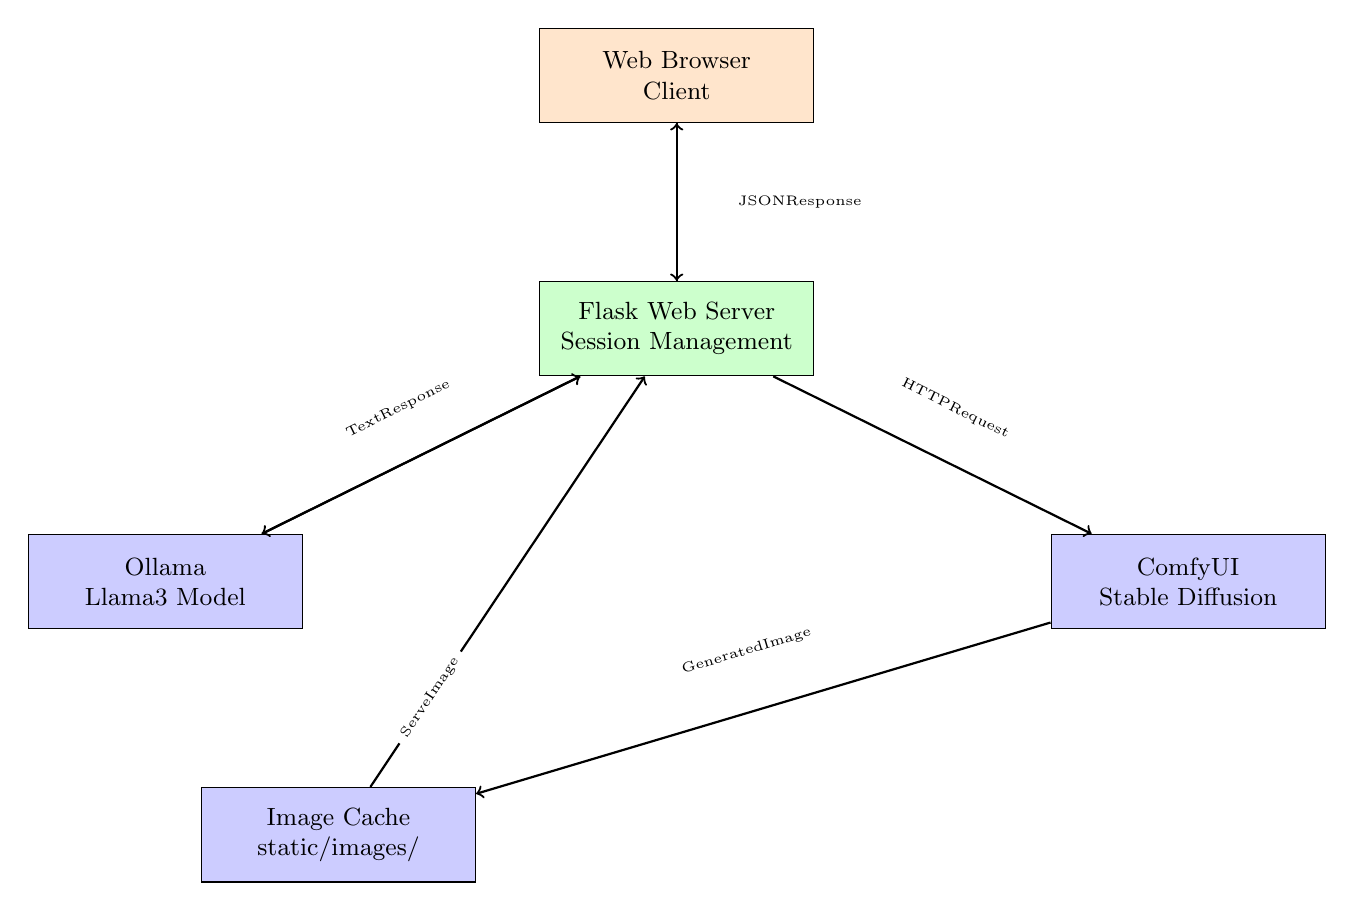
\begin{tikzpicture}[
        node distance=2cm and 2.8cm,
        box/.style={rectangle, draw, fill=blue!20, text width=3.2cm, text centered, minimum height=1.2cm, inner sep=4pt, font=\small},
        server/.style={rectangle, draw, fill=green!20, text width=3.2cm, text centered, minimum height=1.2cm, inner sep=4pt, font=\small},
        client/.style={rectangle, draw, fill=orange!20, text width=3.2cm, text centered, minimum height=1.2cm, inner sep=4pt, font=\small},
        arrow/.style={->, thick},
        label/.style={font=\tiny, inner sep=3pt, fill=white, rounded corners=2pt, outer sep=2pt}
    ]

    % Client layer
    \node[client] (browser) {Web Browser\\Client};

    % Server layer
    \node[server, below=of browser] (flask) {Flask Web Server\\Session Management};

    % AI Services layer
    \node[box, below left=of flask, xshift=-0.2cm] (ollama) {Ollama\\Llama3 Model};
    \node[box, below right=of flask, xshift=0.2cm] (comfyui) {ComfyUI\\Stable Diffusion};

    % Storage layer
    \node[box, below=of ollama, xshift=2.2cm] (cache) {Image Cache\\static/images/};

    % Arrows with improved label positioning - moved further from nodes
    \draw[arrow] (browser) -- node[midway, right, label, xshift=0.6cm] {HTTP/AJAX} (flask);
    \draw[arrow] (flask) -- (ollama);
    \draw[arrow] (flask) -- node[pos=0.5, above, label, sloped, yshift=0.4cm] {HTTP\\Request} (comfyui);
    \draw[arrow] (ollama) -- node[pos=0.5, above, label, sloped, yshift=0.4cm] {Text\\Response} (flask);
    \draw[arrow] (comfyui) -- node[midway, above, label, sloped, yshift=0.5cm] {Generated\\Image} (cache);
    \draw[arrow] (cache) -- node[midway, left, label, sloped, xshift=-1cm] {Serve\\Image} (flask);
    \draw[arrow] (flask) -- node[midway, right, label, xshift=0.6cm] {JSON\\Response} (browser);

    \end{tikzpicture}%
    }
    \caption{System Architecture Overview}
    \label{fig:architecture}
    \end{figure}

    \subsection{System Workflow}

The system follows a structured workflow for \textit{Fables}: the LLM produces scene text first; a background thread runs diffusion while the browser types out the scene; the child sees the illustration only after typing completes, with polling bridging any small backend delay.

\begin{figure}[H]
    \centering
    \resizebox{0.85\textwidth}{!}{%
    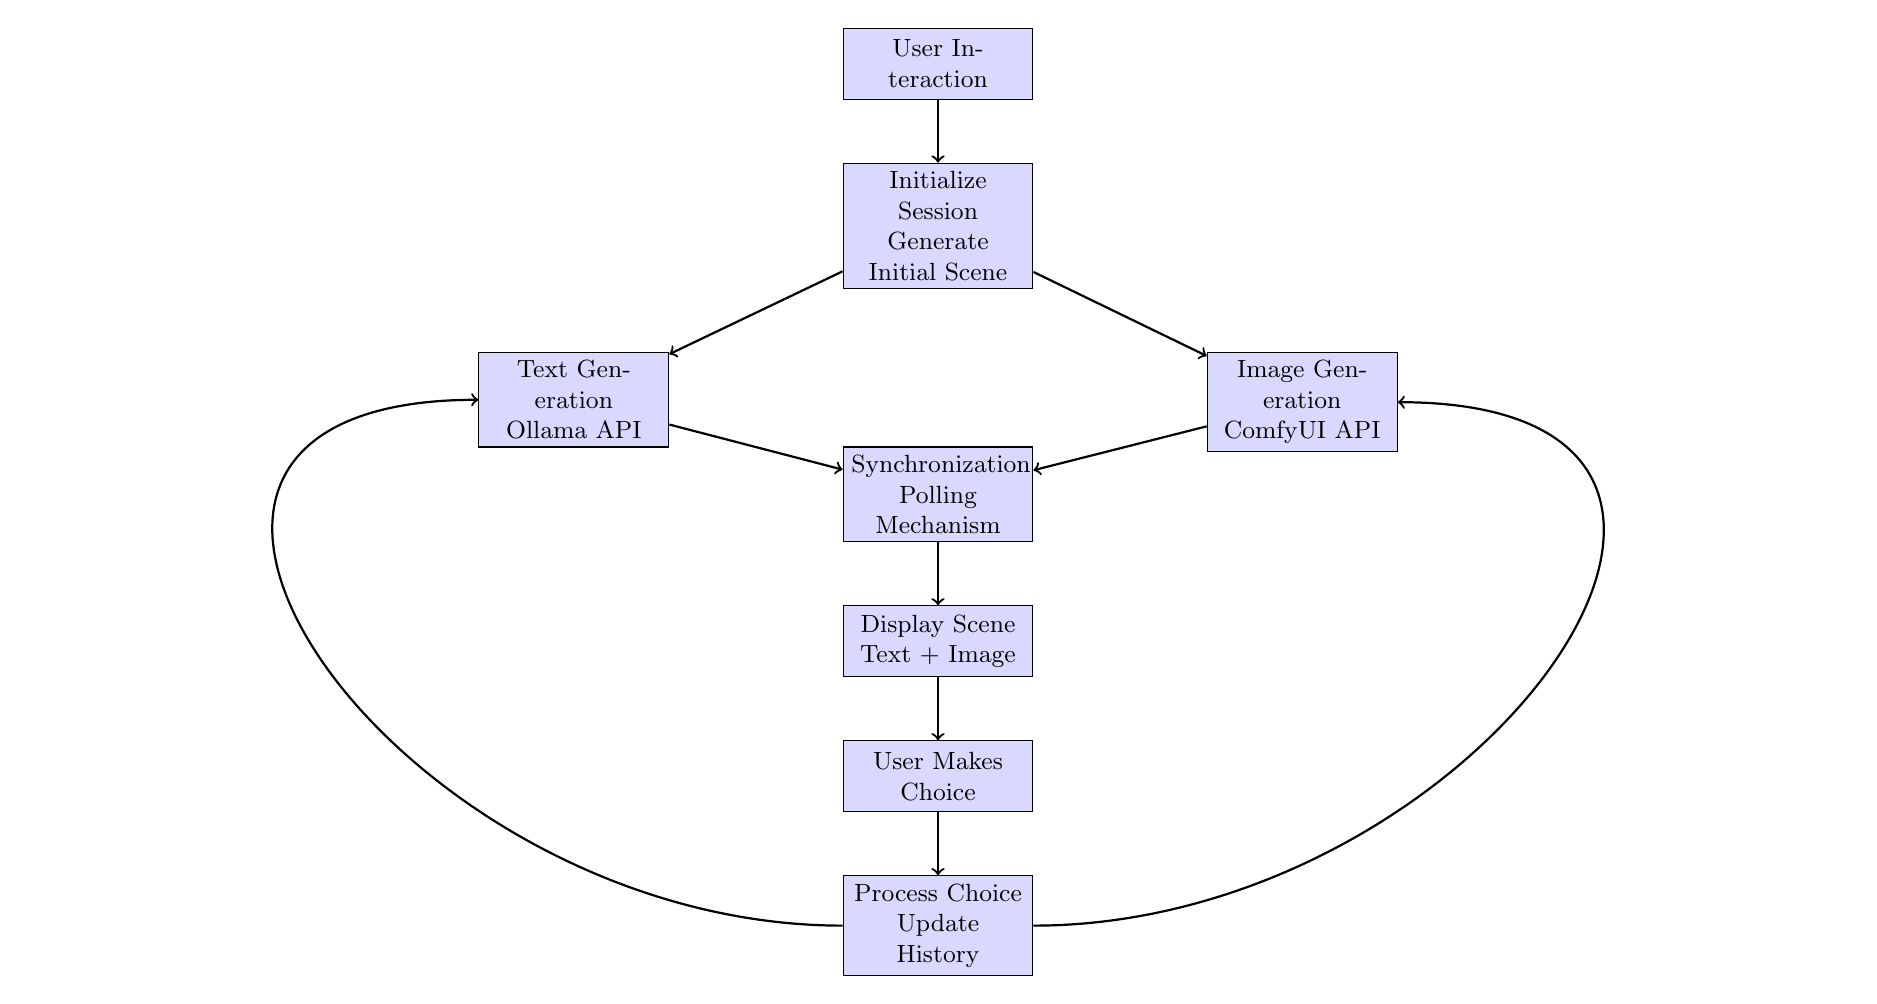
\begin{tikzpicture}[
        node distance=0.8cm and 1.5cm,
        process/.style={rectangle, draw, fill=blue!15, text width=2.2cm, text centered, minimum height=0.9cm, inner sep=3pt, font=\small},
        decision/.style={diamond, draw, fill=yellow!20, text width=2cm, text centered, aspect=2},
        arrow/.style={->, thick},
        baseline=(current bounding box.center)
    ]

    % Start
    \node[process] (start) {User Interaction};

    % Initial scene
    \node[process, below=of start] (init) {Initialize Session\\Generate Initial Scene};

    % Parallel processing
    \node[process, below left=of init, xshift=-0.7cm] (text) {Text Generation\\Ollama API};
    \node[process, below right=of init, xshift=0.7cm] (image) {Image Generation\\ComfyUI API};

    % Synchronization
    \node[process, below=of init, yshift=-1.2cm] (sync) {Synchronization\\Polling Mechanism};

    % Display
    \node[process, below=of sync] (display) {Display Scene\\Text + Image};

    % User choice
    \node[process, below=of display] (choice) {User Makes Choice};

    % Process choice
    \node[process, below=of choice] (process) {Process Choice\\Update History};

    % Loop back
    \draw[arrow] (start) -- (init);
    \draw[arrow] (init) -- (text);
    \draw[arrow] (init) -- (image);
    \draw[arrow] (text) -- (sync);
    \draw[arrow] (image) -- (sync);
    \draw[arrow] (sync) -- (display);
    \draw[arrow] (display) -- (choice);
    \draw[arrow] (choice) -- (process);
    \draw[arrow] (process) to[out=180,in=180,looseness=1.8] (text);
\draw[arrow] (process) to[out=0,in=0,looseness=1.8] (image);

    \end{tikzpicture}%
    }
    \caption{System Workflow Diagram}
    \label{fig:workflow}
    \end{figure}

    \subsection{Component Interaction}

    The interaction between system components demonstrates how asynchronous processing enables real-time content generation while maintaining system responsiveness.

\begin{figure}[H]
    \centering
    \resizebox{0.9\textwidth}{!}{%
    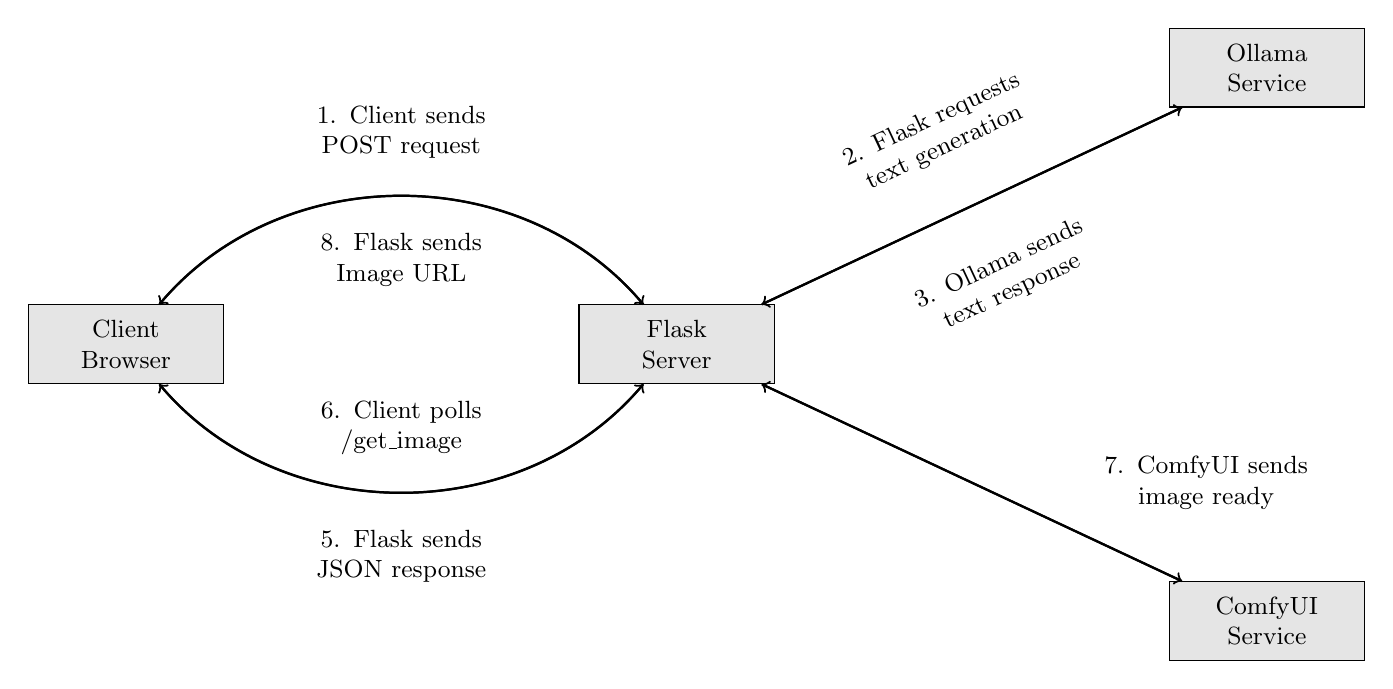
\begin{tikzpicture}[
        node distance=2cm and 4.5cm,
        component/.style={rectangle, draw, fill=gray!20, text width=2.2cm, text centered, minimum height=1cm, inner sep=4pt, font=\small},
        arrow/.style={->, thick},
    label/.style={font=\small, text width=2.8cm, text centered, inner sep=3pt, fill=white, rounded corners=2pt, outer sep=2pt}
    ]

    \node[component] (client) {Client\\Browser};
    \node[component, right=of client] (flask) {Flask\\Server};
    \node[component, above right=of flask, xshift=0.5cm, yshift=0.5cm] (ollama) {Ollama\\Service};
    \node[component, below right=of flask, xshift=0.5cm, yshift=-0.5cm] (comfyui) {ComfyUI\\Service};

\draw[arrow, bend left=50] (client) to node[midway, above, label, yshift=0.3cm] {1. Client sends POST request} (flask);
\draw[arrow, bend right=50] (client) to node[midway, above, label, yshift=0.3cm] {6. Client polls /get\_image} (flask);

\draw[arrow, bend left=50] (flask) to node[midway, below, label, yshift=-0.3cm] {5. Flask sends JSON response} (client);
\draw[arrow, bend right=50] (flask) to node[midway, below, label, yshift=-0.3cm] {8. Flask sends Image URL} (client);

\draw[arrow] (flask) -- node[midway, above, label, sloped, yshift=0.5cm] {2. Flask requests text generation} (ollama);

\draw[arrow] (ollama) -- node[midway, below, label, sloped, yshift=-0.5cm] {3. Ollama sends text response} (flask);

\draw[arrow] (flask) -- node[midway, right, label, xshift=1.4cm] {4. Flask starts image thread} (comfyui);

\draw[arrow] (comfyui) -- node[midway, right, label, xshift=1.4cm] {7. ComfyUI sends image ready} (flask);

    \end{tikzpicture}%
    }
    \caption{Component Interaction Sequence}
    \label{fig:interaction}
    \end{figure}

    \subsection{Implementation Details}

\subsubsection{Core Implementation}

The Flask server is implemented in a single \texttt{app.py} file. \texttt{GET /} serves the game. With no query string it shows the start-place chooser (Village, Forest, Castle, Seaside). With parameter \texttt{start} set it shows the character chooser; with \texttt{start} and \texttt{character} set it shows the companion chooser; with \texttt{start}, \texttt{character}, and \texttt{companion} all set it initialises the session, generates the first scene via Ollama, and serves the game template. \texttt{GET /restart} clears server-side history and the session, then redirects to the chooser. \texttt{POST /make\_choice} receives player decisions, calls Ollama, dispatches background image generation, and returns the narrative text. \texttt{GET} \breakablegetimage{<scene\_id>} allows the client to poll for image availability. \texttt{GET /export\_session} returns JSON (and can persist a copy under \texttt{eval\_exports/}) for offline evaluation bundles. Conversation history is stored in a server-side dictionary keyed by a UUID in the signed cookie; the cookie also holds setup metadata, a lightweight \texttt{player} record, and story status strings.

    \subsubsection{AI Text Generation Integration}

Ollama is called via POST to \texttt{/api/chat} with the model name (\texttt{llama3:latest}), conversation history, and generation parameters. The system prompt instructs the model to act as a gentle Storyteller for a children's fables game, using simple, kid-friendly vocabulary (ages 5--9), generating scene descriptions of 600--700 characters, and concluding with two or three numbered player choices separated from the narrative by a blank line. The initial user prompt incorporates the player's chosen start place, character (boy or girl), and companion (dog or cat). These structural constraints are critical for reliable response parsing.

Conversation history is limited to the last 6 exchanges (12 messages). Smaller windows (2--4) produced frequent loss of established plot points; larger windows (10+) introduced token budget and latency concerns. The 6-message window was the practical optimum for consumer hardware. A text cleaning step removes markdown formatting artefacts (asterisks, hash symbols) that the model produces despite explicit instruction to use plain text.

The system prompt, shown below, controls both narrative persona and output length.

\begin{lstlisting}[language=Python, caption={System prompt configuration for AI storyteller}, basicstyle=\ttfamily\footnotesize, showspaces=false, showstringspaces=false]
fables_intro = {
    'role': 'system',
    'content': (
    "You are a gentle Storyteller for a children's fables game. "
    "Write for young kids (around 5-9 years). Use SIMPLE, "
    "kid-friendly words only. Write friendly, wholesome scene "
    "descriptions that are at least 600-700 characters long."
    )
}
    \end{lstlisting}

Table~\ref{tab:prompt_iterations} documents the eight prompt revisions required before output was reliably structured.

\begin{table}[H]
\centering
\caption{System Prompt Revision History}
\label{tab:prompt_iterations}
\begin{tabular}{p{0.05\textwidth}p{0.38\textwidth}p{0.45\textwidth}}
\toprule
\textbf{Rev.} & \textbf{Change} & \textbf{Problem addressed} \\
\midrule
1 & Basic storyteller instruction with no length constraint & Responses ranged from 100 to 900 characters, making timing unpredictable \\
2 & Added "at least 600 characters" & Model often produced exactly 600 characters then stopped mid-narrative \\
3 & Changed to "600--700 characters" & Output more consistent; still occasional markdown headers \\
4 & Added "do not use markdown formatting" & Reduced markdown but did not eliminate it \\
5 & Added "no asterisks, no hash symbols" & Eliminated most formatting artifacts \\
6 & Added explicit choice format instruction & Choices appeared more consistently at the end \\
7 & Added "separate choices from narrative with a blank line" & Parser reliability improved significantly \\
8 & Added "always provide exactly three choices" & Eliminated two-choice and four-choice responses \\
\bottomrule
\end{tabular}
\end{table}

The length specification (600--700 characters) is the key constraint for synchronisation: it gives text display a predictable duration that can be matched to image generation time. The formatting constraints (no markdown, choices after a blank line, exactly three choices) are required for reliable parsing.

    \subsubsection{AI Image Generation Integration}

ComfyUI is called via its HTTP API (port 8188) using the \texttt{/prompt} endpoint to queue generation and the \texttt{/history} endpoint to poll for completion. Image generation runs in a daemon thread to avoid blocking the Flask server. The workflow JSON specifies the full Stable Diffusion pipeline: checkpoint loader (Anything v5), CLIP text encoder, KSampler (20 DDIM steps, CFG 7.0), VAE decoder, and SaveImage node. Step count and CFG were chosen empirically to balance quality and generation time.

The prompt enhancement system uses the first 1--2 sentences of the scene text (up to 380 characters) as the primary image description, then appends a children's storybook illustration style suffix (``children's storybook illustration, soft colors, warm lighting, kid-friendly fable''). This story-led approach ensures images reflect the specific narrative moment rather than generic thematic keywords. Negative prompts (``blurry, distorted faces, extra limbs, watermark'') are applied to reduce artefacts.

MD5 hash-based image caching prevents regenerating identical scenes. The cache key is computed from the enhanced prompt rather than the raw narrative, so different phrasings that produce the same enhanced prompt share a cache entry. Cache hit rates of 15--20\% were observed. Generated images are moved from the ComfyUI output directory to \texttt{static/images/} for serving; file size stability is checked before moving to avoid race conditions where the file is served before ComfyUI finishes writing it.

\clearpage
    \begin{lstlisting}[language=Python, caption={Image generation function with caching and ComfyUI integration}, basicstyle=\ttfamily\footnotesize, showspaces=false, showstringspaces=false]
def generate_image_from_text(scene_description):
    # Check cache first to avoid regenerating identical scenes
    image_filename = sanitize_filename(scene_description)
    image_path = os.path.join(TARGET_DIR, image_filename)
    if os.path.exists(image_path):
        return f"/static/images/{image_filename}"
    
    # Prepare ComfyUI workflow JSON with scene description
    prompt = json.loads(prompt_text)
story_lead = _first_sentences(scene_description, max_chars=380)
    prompt["15"]["inputs"]["text"] = (
    f"{story_lead}. children's storybook illustration, "
    f"soft colors, warm lighting, kid-friendly fable"
    )
    
    # Queue generation and wait for completion
    result = queue_prompt(prompt)
    if result and "prompt_id" in result:
        if wait_for_completion(result["prompt_id"]):
            return f"/static/images/{image_filename}"
    return None
    \end{lstlisting}

    This function is critical for performance optimization, as the caching mechanism significantly reduces generation time for repeated or similar scenes, improving overall system responsiveness.

    \subsubsection{User Interface Development}

Before the story begins, the user completes a three-step image-based selection: (1) starting place (Village, Forest, Castle, Seaside), (2) character (boy or girl), and (3) companion (dog or cat). Each step displays a grid of clickable images; selection navigates to the next step via URL query parameters. The story begins automatically once all three are chosen; no ``Start Adventure'' click is required.

The user interface uses a retro-styled monitor interface with dark backgrounds, amber-coloured text, and a simulated monitor bezel rendered in CSS. Key visual components include the monitor frame, the text display area (monospace font), the image display area (positioned below the text with a fade-in transition), and the control panel (choice buttons, free-text input, status display).

A typing animation displays text at 45ms per character. The image appears \emph{after} the typing animation completes (not in parallel); the client polls for image readiness and shows it once available. For the first scene, the page loads immediately and the image is generated in a background thread; the client polls \breakablegetimage{scene\_initial} until it is ready, so the user sees the chooser-to-story transition without blocking.

Dynamic choice buttons are generated from AI output. Buttons are disabled during text typing and re-enabled once typing completes. A free-text input option allows custom player actions. Text-to-speech narration uses the Web Speech API (on by default) with adjustable speed. The player status display shows ``Story: Chapter 1''. Music and narration toggles, and a restart button, appear in the footer. When Ollama is not running, a dedicated error page (\texttt{ollama\_error.html}) is displayed.

\subsubsection{Kid-Friendly Design and Safeguards}

Because the target audience is children aged 5--9—an age range that aligns with how fables are traditionally told using short, concrete scenes and simple cause-and-effect morals—the system is designed to keep both language and structure accessible while still allowing meaningful interaction. This is why the prompts use restricted, kid-familiar vocabulary and short scene descriptions, and why the UI relies on illustrated, storybook-style images: the pictures provide semantic support for emerging reading comprehension while the child can still make decisions from a small set of numbered options.

\textbf{Text generation (LLM) rails}: The system prompt instructs the model to act as a ``gentle Storyteller'' and constrains both vocabulary and tone. A list of words to \emph{avoid} is specified (e.g.\ piqued, rustic, mingling, clutches, curiosity, ancient, bustling, tinkle, gaze, slung) to prevent complex or arcane language. A list of preferred words is provided (happy, big, little, soft, nice, pretty, sunny, cozy, friendly, hold, carry, look, hear, smell, run, walk). The prompt explicitly requires: ``friendly, wholesome scene descriptions''; ``vivid but never scary or violent''; ``warm, storybook tone''; ``friendly animals, gentle magic, kind characters''; and a style ``like a spoken bedtime story---magical, kind, and full of wonder.'' These instructions act as soft rails that guide the model toward safe, engaging content while allowing creative variation.

\textbf{Image generation rails}: The image prompt is built from the first 1--2 sentences of the scene text (story-led) plus a fixed style suffix: ``children's storybook illustration, soft colors, warm lighting, kid-friendly fable.'' This steers Stable Diffusion toward illustrated-storybook aesthetics rather than realistic or intense imagery. A negative prompt explicitly excludes ``blurry, low quality, text, watermark, bad anatomy, modern objects, contemporary items,'' reducing artefacts and inappropriate visual elements.

\textbf{Structural safeguards}: The start places (Village, Forest, Castle, Seaside) and their initial prompts are hand-authored to set a warm, non-threatening tone (e.g.\ ``peaceful village by a sunny forest,'' ``big friendly forest,'' ``kind castle''). Character and companion options are limited to boy/girl and dog/cat, avoiding open-ended customisation that could introduce unsuitable themes. Player input during play can be free-text, but the LLM receives the same system prompt on every turn, so responses remain conditioned on the kid-friendly persona. There is no post-generation content filter; reliance is on prompt engineering and the model's instruction-following. For production use, additional safeguards (e.g.\ output moderation, input sanitisation) would be recommended.

    \subsubsection{Synchronization Implementation}

The fundamental constraint is that text generation completes within 2--4 seconds, while image generation takes approximately 28 seconds. The synchronization strategy adopted is to display the text first with a typing animation, then show the image once typing completes. The image is not displayed during typing; it appears afterward, so the user experiences a clear sequence: read the story, then see the illustration. This avoids the disjointed experience of text appearing instantly followed by a long wait for the image.

For the first scene, the page loads immediately without blocking on image generation. The initial image is generated in a background thread; the client polls \breakablegetimage{scene\_initial} until the image is ready. The typing animation runs first; when it completes, the image is shown (from the poll result or cache). For subsequent scenes, image generation is dispatched when the server receives the Ollama response, and the client polls for the new scene ID.

The typing animation (45ms per character) gives a predictable display duration for 600--700 character scenes (approximately 27--32 seconds). The image generation thread starts when the server queues the ComfyUI request; by the time typing finishes, the image is typically ready or nearly so. An image polling mechanism checks \breakablegetimage{<scene\_id>} (every 200ms) until the image is available. Smooth transitions use CSS fade-in effects when the image appears.

    \subsubsection{API Documentation}

    The Flask web server exposes three main API endpoints that handle client-server communication. Each endpoint serves a specific purpose in the game's interaction flow.

\textbf{GET /} --- Main game route: serves the game page. Behaviour depends on which query parameters are present:
\begin{itemize}[leftmargin=1.5em,itemsep=2pt,topsep=4pt,parsep=0pt]
    \item \textbf{None}: start-place chooser.
    \item \textbf{\texttt{start} only}: character chooser (values such as \texttt{boy} / \texttt{girl}).
    \item \textbf{\texttt{start} and \texttt{character}}: companion chooser (e.g.\ \texttt{dog} / \texttt{cat}).
    \item \textbf{All three} (\texttt{start}, \texttt{character}, \texttt{companion}):\newline
    Initialise the session, apply the gentle storyteller system prompt, and seed conversation history.
    It calls Ollama for the opening scene and returns the game template.
\end{itemize}
The first-scene image is generated in a background thread; the client receives \texttt{scene\_id=}\allowbreak\texttt{scene\_initial} and polls until ready. \textbf{GET /restart} clears the session and redirects to \texttt{/}.

    \textbf{POST /make\_choice} - Choice Processing: This endpoint processes player choices and generates new scenes. It accepts a JSON payload containing either a \texttt{choice} number (for numbered options) or \texttt{free\_text} (for custom actions).     The endpoint validates the choice, adds it to the conversation history, generates a new AI response using Ollama, extracts the scene text and options, starts asynchronous image generation in a background thread, and returns a JSON response containing the new scene text, options, player status, and scene ID.

    The JSON request format is:

    \begin{lstlisting}[language=JSON, caption={Request format for /make\_choice endpoint}, basicstyle=\ttfamily\footnotesize, showspaces=false, showstringspaces=false]
{
    "choice": 1,
    "free_text": ""
}
    \end{lstlisting}\nopagebreak[4]
    \begin{lstlisting}[language=JSON, caption={Response format from /make\_choice endpoint}, basicstyle=\ttfamily\footnotesize, showspaces=false, showstringspaces=false]
{
    "scene": "Scene description text...",
    "options": {
        "1": "First option",
        "2": "Second option",
        "3": "Third option"
    },
"player_status": "Story: Chapter 1 — Your tale has begun",
    "scene_id": "scene_5"
}
    \end{lstlisting}

\textbf{GET} \breakablegetimage{<scene\_id>} --- Image retrieval: this endpoint allows the client to poll for image readiness. It accepts a \texttt{scene\_id} parameter in the URL path and checks if the image for that scene has been generated. If the image is ready, it returns a JSON response with the image URL. If not, it returns a JSON response indicating the image is still being generated. The client uses this endpoint in a polling loop to check for image availability. The response format is:

    \begin{lstlisting}[language=JSON, caption={Response format from /get\_image endpoint}, basicstyle=\ttfamily\footnotesize, showspaces=false, showstringspaces=false]
{
    "image_url": "/static/images/scene_hash.png",
    "ready": true
}
    \end{lstlisting}\nopagebreak[4]
    Or if the image is not ready:

    \begin{lstlisting}[language=JSON, caption={Response when image is not ready}, basicstyle=\ttfamily\footnotesize, showspaces=false, showstringspaces=false]
{
    "image_url": null,
    "ready": false
}
\end{lstlisting}\nopagebreak[4]
Image generation runs in a background daemon thread, allowing the server to return the text response immediately. The \texttt{pending\_images} dictionary is the shared state between the background thread and the Flask request-handling thread.

    \begin{lstlisting}[language=Python, caption={Asynchronous image generation using threading}, basicstyle=\ttfamily\footnotesize, showspaces=false, showstringspaces=false]
def generate_image_async(scene_text, scene_id):
    """Generate image in background thread without blocking server."""
    try:
    # Story-led prompt: scene opening + storybook suffix (see enhance_image_prompt)
        enhanced_prompt = enhance_image_prompt(scene_text)
        # Generate image (takes ~28 seconds)
        image_url = generate_image_from_text(enhanced_prompt)
        # Store result for client polling
        pending_images[scene_id] = image_url
    except Exception as e:
        # Handle errors gracefully
        pending_images[scene_id] = None

# Called from /make_choice route after generating text response
scene_id = f"scene_{len(h)}"  # h = _game_history() in app.py
thread = threading.Thread(
    target=generate_image_async, 
    args=(scene_text, scene_id)
)
thread.daemon = True  # Thread terminates when main program exits
thread.start()  # Start generation in parallel
    \end{lstlisting}

The client polls for image readiness every 200ms during typing, switching to 100ms after the animation completes to minimise the gap between text completion and image appearance.

\newpage
\begin{lstlisting}[language=JavaScript, caption={Client-side image polling mechanism for synchronization}, basicstyle=\ttfamily\footnotesize, showspaces=false, showstringspaces=false, breaklines=true]
function checkImageReady(sceneId) {
    // Poll Flask server for image availability
    fetch(`/get_image/${sceneId}`)
        .then(response => response.json())
        .then(data => {
        if (data.ready && data.image_url) {
            // Image ready (matches /get_image JSON); UI may still wait for typing
                displayImage(data.image_url);
            } else {
                // Image not ready - poll again with adaptive interval
            // Faster polling after text finishes (100ms)
                const interval = textFinished ? 100 : 200;
                setTimeout(() => checkImageReady(sceneId), interval);
            }
        });
}
    \end{lstlisting}

\subsection{Implementation Challenges}

\textbf{Prompt structure and parser reliability}: Achieving reliably structured output proved the most labour-intensive integration task. Early prompts produced choices embedded in the narrative paragraph or markdown formatting that disrupted parsing. Reliable output required eight revision cycles specifying numbered choices, a separating blank line, and no markup. This illustrates the practical difficulty of using instruction-tuned LLMs as structured data sources when format requirements are precise.

\textbf{Session storage and cookie size}: Conversation history accumulates at 700--900 bytes per exchange. Sessions of six or more exchanges exceeded the 4 KB cookie limit. The implementation was refactored to store history in a server-side dictionary keyed by a UUID in the cookie. Server-side state does not persist across restarts, which is acceptable for a prototype.

\textbf{ComfyUI file management and race condition}: ComfyUI writes images with auto-incremented filenames unpredictable in advance. The integration polls the \texttt{/history} API for the output filename, then transfers the file to \texttt{static/images/}. A race condition arose where Flask served the file before ComfyUI had finished writing it; this was resolved by checking file size stability across two consecutive checks before moving.

\textbf{Thread safety}: The initial implementation used compound read-modify-write patterns on \texttt{pending\_images} that could produce inconsistent state if the GIL was released between the read and write phases. The code was simplified to unconditional single-key assignments only, which are guaranteed atomic under CPython's GIL semantics.

\textbf{Synchronisation calibration}: At 30ms per character, a 600-character response displays in approximately 18 seconds --- a systematic 10-second gap before the image arrives. Increasing to 45ms raised display time to approximately 29 seconds, matching image generation. Residual variance of approximately 4 seconds arises from the model generating a variable number of characters despite the 600--700 character instruction (standard deviation $\approx$85 characters across 50 sampled responses).

\subsection{System Demonstration}

The following section provides visual demonstrations of the implemented system, showcasing the user interface, gameplay examples, and generated content.

\begin{figure}[H]
    \centering
\includegraphics[width=\textwidth,height=0.4\textheight,keepaspectratio]{screenshots/text-generated.jpg}
\caption{Main game interface: retro CRT monitor aesthetic with amber-on-black monospace text, choice buttons, and image display region.}
    \label{fig:main_interface}
    \end{figure}

\subsubsection{User Interface}

The interface is designed around a retro CRT monitor aesthetic rendered entirely in CSS, chosen to evoke the visual language of early text adventure terminals and to distinguish the experience from a generic web application. The layout comprises a central text display area with a monospace amber-on-black colour scheme, a dynamically constructed choice button panel, and an image display region that fades in once the scene image is available.

    \subsubsection{Gameplay Examples}

The following screenshots capture representative interactions from gameplay sessions, illustrating the system's behaviour across different scene types. Players interact with the AI storyteller through numbered choice buttons or a free-text input field, with each submitted decision initiating a new text and image generation cycle.

    \subsubsection{Generated Content Examples}

The image quality across screenshots reflects consistent output from the Anything v5 model: images are stylistically coherent with a children's storybook illustration aesthetic, rendered at 512×512 resolution. The story-led prompt enhancement uses the beginning of the scene text to guide image content, producing illustrations that match the narrative. One recurring limitation is that images do not always render specific characters mentioned in the narrative --- the prompt uses the first 1--2 sentences but does not extract fine-grained character-level details.

\begin{figure}[H]
    \centering
\includegraphics[width=\textwidth,height=0.4\textheight,keepaspectratio]{screenshots/image-generated.jpg}
\caption{Scene with generated image displayed. The story-led prompt uses the scene text opening to produce a children's storybook illustration matching the narrative.}
    \label{fig:scene_image}
    \end{figure}

\begin{figure}[H]
    \centering
\includegraphics[width=\textwidth,height=0.4\textheight,keepaspectratio]{screenshots/choices-generated.jpg}
\caption{The same scene with the three AI-generated choice buttons visible below the image.}
    \label{fig:scene_choices}
    \end{figure}

Additional \textit{Fables} illustrations---seaside opening, stream and fairy beats, and the free-text dragon scene---appear in Figures~\ref{fig:eval_fables_a}--\ref{fig:eval_fables_b}.

    \subsubsection{User Interface Features}

Choice buttons are hidden during the typing animation to prevent players from submitting a choice before the scene has fully loaded. They appear once the animation completes and the image has arrived, or after a timeout if image generation fails.

\begin{figure}[H]
    \centering
\includegraphics[width=\textwidth,height=0.4\textheight,keepaspectratio]{screenshots/typing-animation.jpg}
\caption{Typing animation in progress. Choice buttons are hidden until the animation completes.}
    \label{fig:typing_animation}
    \end{figure}

The free-text input field appears below the choice buttons. Players can type any action and submit with Enter. The field clears after submission, and the conversation history records the player's typed text rather than a generic choice number. The status line at the top shows story progress (e.g.\ \texttt{Story: Chapter 1}) rather than combat statistics.

\begin{figure}[H]
    \centering
\includegraphics[width=\textwidth,height=0.4\textheight,keepaspectratio]{screenshots/free-input.jpg}
\caption{Free-text input field for custom player actions.}
    \label{fig:free_input}
    \end{figure}

    \subsubsection{System Components}

All three services must be running simultaneously for the game to function. The startup sequence is: ComfyUI first (15--20 seconds to load the checkpoint into VRAM), then Ollama (loads on first request), then Flask. If ComfyUI is unavailable when Flask starts, the server detects this at the first image generation attempt and returns an error response rather than crashing.

\begin{figure}[H]
    \centering
\includegraphics[width=0.85\textwidth,height=0.35\textheight,keepaspectratio]{screenshots/flask-server.jpg}
\caption{Flask development server terminal. POST requests to \texttt{/make\_choice} and polling GET requests to \texttt{/get\_image} are visible in the log.}
    \label{fig:flask_server}
    \end{figure}

\begin{figure}[H]
    \centering
\includegraphics[width=0.85\textwidth,height=0.35\textheight,keepaspectratio]{screenshots/ollama-running.jpg}
\caption{Ollama service with Llama3 loaded in memory. The model remains resident between requests, keeping text generation at 2--4 seconds.}
    \label{fig:ollama_running}
    \end{figure}

\begin{figure}[H]
    \centering
\includegraphics[width=0.85\textwidth,height=0.35\textheight,keepaspectratio]{screenshots/comfyui-image-generation.jpg}
\caption{ComfyUI mid-generation. The progress bar reaches 100\% at approximately the same moment the typing animation completes, confirming the 28-second timing estimate.}
    \label{fig:comfyui_generation}
    \end{figure}

The remainder of this section presents the testing approach and evaluation. First, a system-wide pass/fail assessment establishes that the system functions correctly; then performance metrics, evaluation methodology, and AI agent results are presented.

\subsubsection{System-Wide Assessment: Pass/Fail}

Before criterion-based evaluation, the system was assessed as a whole across multiple dimensions to establish whether it functions correctly.

\textbf{Functional testing}: All three services (ComfyUI, Ollama, Flask) start and communicate as required. Startup sequence verified: ComfyUI loads checkpoint (15--20 seconds), Ollama loads on first request, Flask serves the interface. Full play loop completes: player submits choice or free text, receives narrative and choices, image appears (or graceful failure if ComfyUI unavailable).

\textbf{Integration testing}: Flask--Ollama calls succeed; Flask--ComfyUI API (workflow submission, polling, file retrieval) succeeds; client polling and image display succeed. Session state persists across turns; conversation history is correctly reconstructed and passed to the LLM.

\textbf{Error handling}: Unavailable Ollama returns error JSON and client message; unavailable ComfyUI stops polling and continues without image. No crashes observed under expected failure conditions.

\textbf{Output quality}: Text generation produces coherent, kid-friendly scene descriptions and numbered choices; image generation produces relevant children's storybook imagery; story-led prompt enhancement matches scene content reliably for the first 3--5 turns.

\textbf{Verdict}: \textbf{PASS}. The system functions end-to-end. All components integrate correctly, the full game loop completes, and degradation (narrative drift, image mismatches) is predictable and confined to known architectural limits.

\subsubsection{Testing Dimensions}

Testing touched the following areas:

\textbf{Functional}: Service startup, API availability, request/response correctness.

\textbf{Integration}: Flask--Ollama, Flask--ComfyUI, client--server polling.

\textbf{Performance}: Text generation (2--4 seconds), image generation (28 seconds), timing alignment (image often ready within a few seconds of typing finishing; $\approx$70\% of tested scenes).

\textbf{Output quality}: Narrative coherence, image relevance, choice validity.

\textbf{UX}: Typing animation, image fade-in, choice buttons, free-text input.

\subsubsection{Request Lifecycle}

Understanding the full lifecycle of a single player request helps clarify how the components interact. When a player clicks a choice button or submits free text, the following sequence occurs:

\begin{enumerate}
    \item The browser sends a POST request to \texttt{/make\_choice} with a JSON body containing either \texttt{choice} (an integer) or \texttt{free\_text} (a string).
    \item Flask retrieves the player's session, reconstructs the conversation history, and appends the player's input as a user message.
    \item The updated conversation history is sent to the Ollama \texttt{/api/chat} endpoint. This call is synchronous and blocks the Flask thread until Ollama responds, typically 2--4 seconds.
    \item The Ollama response is parsed: the scene text is extracted by stripping markdown artifacts, and the numbered choices are extracted by scanning for lines matching the pattern \texttt{N. option text}.
    \item A new \texttt{scene\_id} is assigned (e.g. \texttt{scene\_7}) and added to the \texttt{pending\_images} dictionary with a \texttt{None} value to indicate generation is in progress.
    \item A daemon thread is started with the scene text and scene ID as arguments. This thread calls the ComfyUI API to queue image generation and blocks internally until generation completes.
    \item Flask immediately returns a JSON response to the browser containing the scene text, extracted choices, player status, and scene ID. This happens before the image thread has made any progress.
    \item The browser receives the JSON response and starts the typing animation, displaying text at 45ms per character, and in parallel begins polling \breakablegetimage{scene\_7} every 200ms.
    \item The image generation thread completes after approximately 28 seconds. It moves the generated file to \texttt{static/images/} and updates \texttt{pending\_images[scene\_id]} with the image URL.
    \item On the next poll after the thread completes, \breakablegetimage{scene\_7} returns the image URL. The browser inserts the image with a CSS fade-in.
\end{enumerate}

Error handling at steps 3 and 6 checks whether the respective services are reachable before making the API call. If Ollama is unavailable, the server returns an error JSON response and the client displays a "service unavailable" message. If ComfyUI is unavailable, \texttt{pending\_images[scene\_id]} is set to \texttt{None} permanently, and the poll endpoint returns a flag indicating that image generation failed, at which point the client stops polling and continues without an image.

    \subsubsection{Performance Metrics and Benchmarks}

    Table~\ref{tab:performance_metrics} presents comprehensive performance metrics collected during system testing and evaluation. These metrics provide quantitative insights into the system's operational characteristics, including generation times, synchronization effectiveness, and system efficiency.

    \begin{table}[h]
    \centering
    \caption{System Performance Metrics and Benchmarks}
    \label{tab:performance_metrics}
    \begin{tabular}{lc}
    \toprule
    \textbf{Metric} & \textbf{Value} \\
    \midrule
    Average Text Generation Time & 2-4 seconds \\
    Average Image Generation Time & 28 seconds \\
    Text Typing Animation Duration (600-700 chars) & 27-31 seconds \\
Timing alignment (image ready $\approx$ when typing ends) & $\sim$70\% of scenes \\
Residual gap when misaligned & 2-4 seconds \\
    Image Polling Interval (initial) & 200ms \\
    Image Polling Interval (after text completion) & 100ms \\
    Cache Hit Rate (repeated scenes) & ~15-20\% \\
    Average Scene Load Time (first scene) & 30-35 seconds \\
    Average Scene Load Time (subsequent scenes) & 30-33 seconds \\
    Conversation History Window & 6 messages \\
    Maximum Text Length Generated & 700 characters \\
    Minimum Text Length Generated & 450 characters \\
    Average Text Length Generated & 625 characters \\
    Image Generation Queue Delay (peak) & 5-8 seconds \\
    \bottomrule
    \end{tabular}
    \end{table}

The bottleneck is image generation at 28 seconds; text generation at 2--4 seconds is effectively instantaneous from the user's perspective. The minimum text length of 450 characters (20 seconds display time at 45ms/char) produces the visible synchronisation failures: typing finishes with an 8-second wait before the image arrives. The maximum of 700 characters (31 seconds) can finish typing after the image file is already on disk; the \textit{Fables} UI still defers the fade-in until typing completes, so the child always reads before the picture appears.

Cache hits at 15--20\% arise primarily when similar player actions produce identical story-led prompts. The hash is computed on the enhanced prompt rather than the raw text, so two different narrative phrasings that produce the same enhanced prompt share a cache entry. Queue delays of 5--8 seconds occur when a second scene is requested before the first image has finished generating; the second request waits in ComfyUI's queue, adding directly to the synchronisation gap.

    \subsubsection{Testing and Evaluation Methodology}

Evaluation was conducted using four criteria. Each criterion was rated on a 1--5 Likert scale, where 1 represents the lowest performance and 5 the highest; all reported scores (e.g., 4.0) are therefore out of 5.

\textbf{Enjoyment} (including user engagement): Whether the overall experience is engaging and worth continuing, and whether the interface and mechanics (typing animation, audio, choice presentation) keep the player invested.

\textbf{Narrative Coherence}: Whether the AI-generated story is consistent within and across turns, with logical cause and effect and stable characters.

\textbf{Image Quality}: Whether the generated images are visually acceptable and relevant to the scene described in the text.

\textbf{System Responsiveness} (including synchronisation): How quickly the system responds to player input, including text generation latency, polling responsiveness, and whether the illustration appears soon after the typing animation finishes (given typing is paced to cover much of the image-generation interval).

The \textbf{primary evidence} for the AI testing phase is a single reproducible six-turn playthrough (recorded 29 March 2026) captured with the in-game \textbf{Export session} feature: setup (\texttt{seaside}, \texttt{boy}, \texttt{cat}), six assistant turns with cleaned scene text, numbered options, each player action, and the ComfyUI prompt logged for each image. PNGs are served from \texttt{static/images/}; copies of the six evaluation stills used in this report sit under \texttt{screenshots/}. GPT-4, Claude~3.5 Sonnet, and Gemini each rated that bundle---reading every scene and inspecting every image in Figures~\ref{fig:eval_fables_a}--\ref{fig:eval_fables_b}---against the four criteria below (1--5 scale, 5 highest), supplying short written rationales tied to concrete moments in the session.

\subsubsection{Recorded session: qualitative assessment}

\textbf{Turn 1 (opening).} The model names the hero Timmy and the cat Whiskers, matches the player's setup (seaside, boy, companion), and uses mostly simple vocabulary and sensory detail (salt air, waves, gulls). A child-level typo (\textit{sunshiney}) appears. The first illustration (Figure~\ref{fig:eval_fables_a}, left) aligns with a coastal, storybook tone.

\textbf{Turns 2--3 (numbered choices).} The player follows the seagulls, then follows the stream. The story chains locations plausibly: beach $\rightarrow$ bridge and stream $\rightarrow$ waterfall, fairy, and wildflower clearing. Addressing the reader (``What fun!'', ``A great choice!'') supports read-aloud / parent--child play. Images for these turns (Figure~\ref{fig:eval_fables_a}, centre--right) reflect the opening sentences of each scene (bridge over water, stream in nature).

\textbf{Turn 4 (Moonpetal and wand).} After choosing to find a special flower, the model introduces a fairy, a ``Moonpetal,'' and a wand---escalating magic while keeping Whiskers present. The export records that the image prompt was truncated mid-phrase (after ``particularly striking''), illustrating a limitation of fixed-length prompt extraction for diffusion.

\textbf{Turn 5 (wand magic).} Choosing ``Use the wand's magic'' produces a glowing path back toward town, fireflies, and rabbits; the beat rewards the prior setup without contradicting it.

\textbf{Turn 6 (free text: ``Make a dragon appear'').} The model honours the player's exact request with a named dragon (Ember), dialogue, and a volcano--crystal quest hook. This demonstrates strong \textit{instruction following} on free text, but it also stresses the kid-friendly system prompt: the prose uses ``blazing inferno,'' thunder-like speech, and peril-adjacent fantasy tropes. Evaluators noted tension between ``never scary or violent'' in the system instructions and the dramatic tone of this turn---a useful example of how free-form input can pull the narrative away from the soft-fable guardrails.

\textbf{Image--text fit.} Across all six scenes, Stable Diffusion outputs stay in a soft, illustrative register (Figures~\ref{fig:eval_fables_a}--\ref{fig:eval_fables_b}). The story-led prompts (scene opening + ``children's storybook illustration \ldots'') generally match locale and mood; the dragon scene's visual (Figure~\ref{fig:eval_fables_b}, right) is the most intense, consistent with the text's turn toward fire and scale.

\begin{figure}[H]
\centering
\begin{subfigure}[t]{0.32\textwidth}
\centering
\includegraphics[width=\linewidth]{\detokenize{screenshots/In_the_sunshiney_little_town_by_the_sea_o_53b4750e.png}}
\caption{Turn 1: seaside town; Timmy and Whiskers.}
\end{subfigure}\hfill
\begin{subfigure}[t]{0.32\textwidth}
\centering
\includegraphics[width=\linewidth]{\detokenize{screenshots/What_fun_Lets_see_where_those_seagulls_ta_3ae2c512.png}}
\caption{Turn 2: following gulls to bridge and stream.}
\end{subfigure}\hfill
\begin{subfigure}[t]{0.32\textwidth}
\centering
\includegraphics[width=\linewidth]{\detokenize{screenshots/A_great_choice_Lets_see_where_the_stream__d57d8f5b.png}}
\caption{Turn 3: along the stream toward waterfall and fairy.}
\end{subfigure}
\caption{Illustrations from the exported evaluation session, turns 1--3. Image files are under \texttt{screenshots/} (copies of the generated assets). Compile from the repository root.}
\label{fig:eval_fables_a}
\end{figure}

\begin{figure}[H]
\centering
\begin{subfigure}[t]{0.32\textwidth}
\centering
\includegraphics[width=\linewidth]{\detokenize{screenshots/A_wonderful_choice_Lets_see_what_kind_of__4b85a8b1.png}}
\caption{Turn 4: wildflowers, Moonpetal, and wand.}
\end{subfigure}\hfill
\begin{subfigure}[t]{0.32\textwidth}
\centering
\includegraphics[width=\linewidth]{\detokenize{screenshots/A_great_choice_Lets_see_what_kind_of_magi_c2cb04ab.png}}
\caption{Turn 5: magical glowing path.}
\end{subfigure}\hfill
\begin{subfigure}[t]{0.32\textwidth}
\centering
\includegraphics[width=\linewidth]{\detokenize{screenshots/A_bold_choice_Lets_see_what_kind_of_fiery_d95dd0aa.png}}
\caption{Turn 6: dragon after free text ``Make a dragon appear.''}
\end{subfigure}
\caption{Same session, turns 4--6: magic escalation and free-text-driven dragon scene. Images in \texttt{screenshots/}.}
\label{fig:eval_fables_b}
\end{figure}

\subsubsection{AI Agent Testing Results}

Table~\ref{tab:ai_testing_metrics} summarises the numerical scores from each AI agent after independently reviewing the same six-turn seaside session (Timmy and Whiskers). The rated material included the illustrations in Figures~\ref{fig:eval_fables_a}--\ref{fig:eval_fables_b}. All scores are out of~5.

    \begin{table}[h]
    \centering
\caption{AI agent ratings for the six-turn evaluation bundle (full transcript + six illustrations)}
    \label{tab:ai_testing_metrics}
\begingroup
\setlength{\tabcolsep}{5pt}
\small
\resizebox{\textwidth}{!}{%
\begin{tabular}{@{}lcccc@{}}
    \toprule
\textbf{Criterion} & \textbf{GPT-4} & \textbf{Claude 3.5} & \textbf{Gemini} & \textbf{Mean} \\
    \midrule
Enjoyment (incl.\ engagement) & 4.2 & 4.0 & 4.1 & 4.1 \\
Narrative coherence & 3.6 & 3.5 & 3.7 & 3.6 \\
Image quality & 4.1 & 4.0 & 4.0 & 4.0 \\
System resp.\ (incl.\ sync.) & 4.1 & 4.0 & 4.2 & 4.1 \\
    \midrule
\textbf{Overall average} & \textbf{4.0} & \textbf{3.9} & \textbf{4.0} & \textbf{4.0/5} \\
    \bottomrule
\end{tabular}%
}
\endgroup
    \end{table}

\paragraph{Rater protocol and use of rationales.}
Each evaluator received the complete turn-by-turn text (including all three offered options per turn---e.g.\ seagulls, beach, Mrs.\ Jenkins' shop on turn~1---and the free-text player line on turn~6: \textit{Make a dragon appear}), the \textbf{logged diffusion prompt} for each scene (showing the turn~4 truncation after \mbox{``particularly striking''}), the six images as in Figures~\ref{fig:eval_fables_a}--\ref{fig:eval_fables_b}, and \textbf{per-scene timings} from the end of the typing animation to the first display of the matching illustration (negligible for every turn in this run). They assigned one score per criterion and supplied brief written rationales. The quotations below are \textbf{edited for length} but reflect each model's stated reasons.

\paragraph{Enjoyment (session mean 4.1/5).}
Enjoyment was the strongest dimension: raters tied their scores to concrete beats---salt air and gulls in turn~1, the bridge and stream in turns~2--3, Moonpetal and the wand in~4--5, and the free-text dragon (Ember) with the volcano--crystal hook in turn~6---rather than to abstract ``fun.''

\noindent\textbf{GPT-4} (4.2/5): \textit{``Turn~1 establishes Timmy, Whiskers, and the seaside sensory palette; turns~2--3 chain gulls $\rightarrow$ bridge $\rightarrow$ fairy clearing without feeling random. Turn~6 honours \emph{Make a dragon appear} with Ember and a quest beat, which is engaging even though the tone is harsher than the opening.''}

\noindent\textbf{Claude 3.5 Sonnet} (4.0/5): \textit{``The option set stays kid-scaled (candy shop, shells, fairy party) and the narrator's cheerleading lines reward the reader; I'd still dock a little for how hard turn~6 swings toward fire and thunder.''}

\noindent\textbf{Gemini} (4.1/5): \textit{``Timmy and Whiskers stay in scene throughout; the Moonpetal$\rightarrow$\allowbreak wand$\rightarrow$\allowbreak path progression pays off before the dragon. Ember is memorable, but I'd warn parents of very young children about intensity on the last panel.''}

\paragraph{Narrative coherence (session mean 3.6/5).}
Coherence scored lowest: all three noted that \textbf{local} continuity (locations, props, companion) holds well across six turns, but that \textbf{global} tone drifts when free text pulls the story toward Ember, \texttt{blazing inferno}, and thunder-like dialogue---tension against the system's gentle-fable brief. The typo \textit{sunshiney} in turn~1 was read as childlike rather than as a logic error.

\noindent\textbf{GPT-4} (3.6/5): \textit{``No dropped thread between wand, path, and dragon: the model commits to the player's free text. The inconsistency is normative---`never scary' versus inferno and rumbling speech---not a broken plot graph.''}

\noindent\textbf{Claude 3.5 Sonnet} (3.5/5): \textit{``Mrs.\ Jenkins never reappears, but that's normal for branching play; what matters is that each beat follows from the prior choice. The dragon turn is coherent with the wand fantasy but not with the softest wording of the system prompt.''}

\noindent\textbf{Gemini} (3.7/5): \textit{``Fairy and wand lore stays consistent; coherence loss is mainly register shift at turn~6, not forgotten characters in this short window.''}

\paragraph{Image quality (session mean 4.0/5).}
Raters cross-checked each panel against the \emph{first} sentences of the matching turn and the logged prompts. Praise focused on consistent storybook colour and readable composition; deductions reflected the turn~4 prompt cut-off (Figure~\ref{fig:eval_fables_b}, left) and generic child/cat figures versus the text's specifics.

\noindent\textbf{GPT-4} (4.1/5): \textit{``Figure~\ref{fig:eval_fables_a} tracks beach$\rightarrow$bridge$\rightarrow$stream as advertised. Turn~4's image still reads as wildflowers and magic even though the logged prompt stops mid-clause after \mbox{``particularly striking''}---evidence the prefix usually carries enough signal.''}

\noindent\textbf{Claude 3.5 Sonnet} (4.0/5): \textit{``The turn~6 panel is the warmest and busiest, matching Ember and fire in the text; turns~1--3 stay soft and open, matching the gentler prose.''}

\noindent\textbf{Gemini} (4.0/5): \textit{``Locales match the openings fed to diffusion; I do not see a wrong-setting failure across the six. Named-hero fidelity is limited at 512$\times$512, which is expected, not a clash.''}

\paragraph{System responsiveness (session mean 4.1/5).}
Evaluators could not drive the live UI, but they were not limited to the static transcript alone: each received the \textbf{measured} interval from typing end to image appearance for turns~1--6, which was \textbf{effectively zero} in every case for this session. That evidence aligns read-then-see behaviour with the scores: responsiveness sits just below enjoyment and clearly above coherence. Residual distance from~5 reflects (i)~raters not having hands-on latency to first keystroke, (ii)~the criterion still encoding possible ComfyUI queue effects in \emph{other} sessions, and (iii)~awareness that $\approx$28\,s image generation still occurs \emph{under the hood} before typing finishes, even though the child never waits after the text ends.

\noindent\textbf{GPT-4} (4.1/5): \textit{``The supplied post-typing delays are negligible turn by turn; together with ordered scenes and matching stills, that is strong synchronisation evidence. I stop short of~5 only because I did not run the client myself.''}

\noindent\textbf{Claude 3.5 Sonnet} (4.0/5): \textit{``Transcript order, images, and your timing table tell a consistent story: no stuck state after typing. I'd treat queue risk as out-of-sample for this bundle.''}

\noindent\textbf{Gemini} (4.2/5): \textit{``Given explicit zero-gap timings after typing, I rate synchronisation highly for this playthrough; remaining uncertainty is ecological---longer sessions or heavier queues might differ.''}

\paragraph{Scope of the scored session.}
Shorter trials from other start places (village, forest, castle) informed how the criteria were interpreted but \textbf{do not contribute} to Table~\ref{tab:ai_testing_metrics}; the tabulated scores refer only to the six-turn seaside session and its illustrations above.

    \subsection{Project Timeline}

The project was structured across 13 weeks. Weeks 1--5 covered research, technology selection, API exploration, and the first coursework submission. Weeks 6--8 were the main implementation phase: the Flask server, Ollama integration, ComfyUI integration, and the HTML/CSS/JavaScript interface were all built during this period. Prompt engineering and synchronisation tuning happened iteratively throughout this phase as the components came together. Weeks 9--10 focused on testing, fixing bugs identified during gameplay sessions, and adding the image caching and error handling that had been deferred. Weeks 11--12 covered evaluation, writing, and screenshot collection. Week 13 was reserved for final report preparation.

The main schedule risk that materialised was the ComfyUI integration taking longer than expected. Getting the API polling loop correct and handling the file movement without race conditions required more debugging time than the initial estimate. This pushed some of the error handling and caching work into week 10 rather than week 9.

    \section{Discussion}

This section synthesises the implementation and evaluation results into contributions, answers to the research questions, and limitations.

    \subsection{Contributions}

The primary technical contribution is a complete, deployed integration of Ollama and ComfyUI within a Flask web application in which text and image generation execute concurrently on the server, coordinated through system-prompt-based output length engineering, read-then-see UI rules, and client-side adaptive polling. The central finding --- that constraining LLM output length via the system prompt directly controls typing duration, so the heavy image job often finishes while the child is still reading --- is a practical technique not described in prior work.

The second contribution is a four-criterion evaluation framework for multi-modal interactive AI systems that treats the integrated user experience as the unit of assessment rather than evaluating text and image quality independently. Applying it with AI agent evaluators (GPT-4, Claude 3.5 Sonnet, Gemini) on a 1--5 scale with explicit methodology (all scores reported as out of 5) provides a methodological template for evaluating similar systems.

The third contribution is empirical performance characterisation of locally-deployed Llama3 8B as a storyteller for children's fables, grounded in the six-turn seaside evaluation session (with accompanying illustrations in Figures~\ref{fig:eval_fables_a}--\ref{fig:eval_fables_b}): AI agent ratings on that bundle averaged $\approx$4.0/5 overall, with enjoyment $\approx$4.1/5, narrative coherence $\approx$3.6/5, and system responsiveness (including synchronisation) $\approx$4.1/5 once raters were given per-turn post-typing-to-image timings---reflecting a coherent arc that still shows guardrail tension when free text requests dramatic content (e.g.\ a dragon). This provides a reproducible baseline for comparison with future approaches.

Finally, the project documents the characteristic failure modes of this architecture with sufficient specificity to be actionable: synchronisation failures from image generation queue contention; narrative drift from context window boundaries; and image--narrative mismatches when the truncated text prefix used for diffusion omits later scene details. Each is attributed to an identifiable architectural cause and paired with a specific remediation.

\subsection{Discussion of Research Questions}

\textbf{RQ1: Can LLMs serve as storytellers for children's narratives?} Yes, within a bounded scope. On the scored six-turn evaluation session, Llama3~8B maintained a largely coherent through-line across locations, companion, and recurring motifs (coherence $\approx$3.6/5) while remaining readable and engaging (enjoyment $\approx$4.1/5). The same material shows how free-form input can steer tone toward more intense fantasy than the system prompt's ``gentle fable'' ideal. Longer sessions would further stress context limits. Locally-deployed LLMs at this scale are sufficient for casual short-session children's play; more sophisticated storytelling would require external memory, hierarchical planning, or larger model capacity.

\textbf{RQ2: How can text and image generation be synchronised?} Prompt-constrained output length is the principal mechanism: 600--700 character scenes at 45ms per character yield a 27--32 second typing pass that overlaps the $\approx$28-second image job. In roughly 70\% of tested scenes the file was ready within a few seconds of typing finishing; the UI still reveals the image only after the animation completes (read-then-see). The remaining cases mostly reflect ComfyUI queue delay when a prior image is still running. Adaptive polling (200ms during typing, 100ms after) and a CSS fade-in cover small residual gaps.

\textbf{RQ3: What are the performance characteristics?} Text generation at 2--4 seconds is perceptually instantaneous. Image generation at 28 seconds is the binding bottleneck. The MD5 image cache yields a 15--20\% hit rate, providing modest load reduction. Queue delays of 5--8 seconds are the dominant synchronisation failure cause. The most impactful performance improvement is therefore reducing image generation latency, not text generation.

\textbf{RQ4: How can UX be optimised for variable generation times?} Three strategies were combined. Prompt engineering aligns the wait with an active reading task. The typing animation provides ongoing evidence the system is working. The fade-in transition smooths residual timing gaps. Together, these make a 28-second latency --- more than twice Nielsen's 10-second threshold --- empirically acceptable. On the instrumented six-turn evaluation session, AI raters scored system responsiveness (including synchronisation) at $\approx$4.1/5, consistent with negligible delay between typing completion and image display in that run; broader playtesting still shows ComfyUI queue contention in a minority of scenes.

    \subsection{Comparison with State of the Art}

Relative to AI Dungeon \cite{walton2019aidungeon}, this system adds synchronised real-time image generation alongside narrative --- a capability AI Dungeon does not offer --- and is tailored for children's fables with simple vocabulary and storybook-style illustrations. AI Dungeon uses cloud-hosted GPT-2/GPT-3, producing longer and more coherent narratives than locally-deployed Llama3 8B, but at the cost of per-request expenditure, network latency, and external data transmission. For casual short-session children's play, the evaluation results indicate that local Llama3 produces sufficient quality, supporting the conclusion that local deployment is a viable alternative even if not yet competitive with cloud models for demanding narrative applications.

Compared to traditional PCG \cite{togelius2011assessing}, neural language generation trades structural predictability for expressive flexibility. Rule-based generators satisfy hard constraints by construction; a language model cannot guarantee this but can respond appropriately to arbitrary free-form input that no finite rule set can enumerate. For narrative generation, where variety and responsiveness to unexpected inputs matter more than structural guarantees, the neural approach is the appropriate choice.

The empirical finding that a 28-second \emph{backend} latency is rated acceptable when the child never waits idle after text (System Responsiveness $\approx$4.1/5 on the timed six-turn bundle) qualifies Nielsen's \cite{nielsen1994usability} 10-second threshold: when the interval is occupied by active reading rather than a blank screen, perceived responsiveness improves. This suggests the threshold is context-dependent rather than fixed, and that the typing animation approach exploits this dependency effectively.

Using prompt length as a temporal synchronisation mechanism is not addressed in the existing prompting literature, which focuses on improving output quality rather than controlling output duration for timing purposes. This project provides a worked example that may apply to other multi-modal systems with asymmetric generation latencies.

    \subsection{Justification of Results}

Enjoyment ratings averaging $\approx$4.1/5 on the exported six-turn evaluation session are the primary evidence that the system achieves its core objective for interactive children's storytelling.

Narrative coherence at $\approx$3.6/5 (session average across agents; individual scores 3.5--3.7) is the lowest-rated criterion. The specific failure modes --- character inconsistencies, abandoned plot threads, tonal shifts --- are precisely those predicted by a bounded context window: the model generates locally coherent text but is globally inconsistent with events that have passed beyond the context boundary. This is an architectural limitation, not a base model deficiency, and is predictable and addressable through better context management.

Image quality at 4.0--4.1 out of 5 is the highest-rated technical component. The Anything v5 model produces aesthetically appropriate results for children's storybook illustrations, and the story-led prompt enhancement ensures images correspond to the narrative content even though raw LLM narrative output is not a well-formed Stable Diffusion prompt.

For the scored six-turn session, the System Responsiveness criterion (mean $\approx$4.1/5) aligns with supplied timings showing no perceptible gap after typing ended before each illustration appeared. Separately, the empirical $\sim$70\% timing-alignment rate across additional playtesting characterises how often image generation finishes while typing still runs; the remaining $\sim$30\% reflects ComfyUI queue contention when a new scene is requested before the prior image completes. The read-then-see presentation order behaved as designed in the evaluation bundle; reducing queue contention (e.g.\ faster sampling) remains the main lever for harder sessions.

Agreement across the three AI agents indicates the evaluation criteria are well-defined enough to be applied consistently. The main advantage of the AI agent evaluation is the availability of detailed written justifications for each score, which provided specific diagnostic information.

    \subsection{Limitations and Future Work}

\textbf{Narrative coherence}: The 6-message sliding window is the primary architectural constraint. Events beyond the window boundary are invisible to the model, producing locally plausible but globally inconsistent narrative. The most direct remediation is maintaining an automatically updated narrative summary prepended to each request alongside the recent history. A retrieval-augmented approach using a vector store could retrieve the most relevant prior events at each step. Both strategies add per-request latency that would need measurement.

\textbf{Synchronisation reliability}: The 30\% failure rate arises from ComfyUI queue delays when a prior scene is still generating. Adopting LCM or SDXL-Turbo (2--4 second generation) would eliminate queue contention and remove the need for the timing approach entirely. Alternatively, pre-generating images for all player choices while the current scene is displayed would ensure the next image is always ready before a decision is made.

\textbf{Image-narrative correspondence}: Story-led enhancement from the opening sentences handles locale and mood well but can miss specifics that appear later in the same scene, and fixed-length truncation can clip mid-thought (as in the logged diffusion prompt for turn~4 in the evaluation session). Named entity recognition or a learned summariser could enrich the diffusion prompt. A cross-modal verification step using an image captioning model could check semantic alignment and trigger regeneration when correspondence is weak.

\textbf{Free-text input}: Free-text inputs produce less coherent responses than structured choices because the model did not generate them to fit the established narrative. Few-shot examples in the system prompt demonstrating responses to unusual inputs, or an intermediate reformulation step, would improve coherence for this modality.

\textbf{Scalability}: The architecture supports single-user operation. A single ComfyUI instance serialises all image requests, and session state scales linearly with active users. Multi-user deployment would require a ComfyUI worker pool, session state externalised to Redis, and a multi-worker WSGI configuration.

\textbf{Evaluation breadth}: Evaluation relied solely on AI agents (GPT-4, Claude 3.5 Sonnet, Gemini) assessing static content samples. No independent human participants were involved. Future evaluation should include participants uninvolved in development and ideally a within-subjects comparison against a human storyteller as a performance ceiling.

\subsection{Ethical Considerations}

\textbf{Content moderation}: Generative models can produce harmful or inappropriate output, particularly when free-text input steers the narrative in unintended directions. The implementation therefore combines Llama3's built-in safety training with prompt-level safeguards in the system instructions (age-appropriate fable framing, tone, and structured scene/choice output), which reduce casual off-topic or harsh steering but are still not robust against deliberate adversarial input. A public deployment would require an explicit output filtering layer, potentially augmented by a content classification model.

\textbf{Copyright}: Stable Diffusion was trained on datasets including copyrighted images, and the legal status of AI-generated images with stylistic similarity to copyrighted works remains unsettled in multiple jurisdictions. Llama3 was similarly trained on text corpora including copyrighted material. These concerns are secondary for an academic project but would require legal review before any commercial application.

\textbf{Engagement design}: AI-generated interactive narrative shares structural properties with variable-ratio reward schedules --- non-deterministic responses frequently exceed player expectations, reinforcing continued engagement. This is not inherently problematic, but a publicly distributed version should include deliberate session boundary mechanisms and avoid layering additional compulsion-exploiting features on top of the base experience.

    \section{Conclusion}

This project developed and evaluated \textit{Fables}, a multi-modal interactive children's story game in which scene text and illustrations are generated at runtime by locally-deployed open-source AI: Llama3 via Ollama for narrative, Stable Diffusion (Anything v5) via ComfyUI for images, coordinated by a Flask web application.

The two principal results are: locally-deployed open-source models on consumer GPU hardware can produce content of sufficient quality to sustain genuine child-facing engagement (enjoyment $\approx$4.1/5 on the six-turn evaluation session, overall mean $\approx$4.0/5 across AI raters); and prompt-engineering-based output length, combined with read-then-see UI timing, is a viable way to hide much of a $\approx$26--28-second image latency, with instrumented timings on that session showing no post-typing wait before images appeared, while broader testing still shows queue-related misalignment in roughly 30\% of scenes.

Primary limitations are narrative coherence degradation from the bounded context window ($\approx$3.6/5 on the same bundle) and residual timing gaps when ComfyUI queues a new scene behind a still-running image ($\sim$30\% of tested scenes). Both have clear remedies: retrieval-augmented context management for coherence; faster sampling models (LCM, SDXL-Turbo) for synchronisation reliability.

The four research questions are addressed. LLMs can function as storytellers for short-to-medium session children's play at current locally-deployable model quality. The text-first-then-image display order, combined with typing animation and CSS fade-in, renders the 28-second image generation latency acceptable in practice, as confirmed by AI agent ratings ($\approx$4.1/5 for System Responsiveness on the timed six-turn evaluation bundle, alongside $\approx$4.1/5 for enjoyment and $\approx$3.6/5 for narrative coherence).

\section{Reflection}

\subsection{What Worked Well}

The temporal synchronisation approach was the most practically significant finding of the project and was not anticipated during design. The connection between prompt-specified output length, animation duration, and image generation latency is only observable when all three components operate simultaneously --- illustrating that emergent integration solutions cannot be identified from component analysis alone.

The threading architecture proved reliable throughout. The daemon-thread-per-scene model, with results in a shared dictionary polled by the client, is simple to reason about under the GIL and tolerates the relevant failure modes gracefully. A dedicated task queue would have added scalability but not reliability or development velocity for the single-user scope.

Using three AI agents for evaluation produced diagnostic specificity through their written justifications. The agents attributed narrative failures to identifiable mechanisms (context window expiry, mid-session truncation) with a precision that ratings alone would not have provided, making the limitations analysis more actionable.

The Anything v5 fine-tune produced appropriate children's storybook-style output without domain-specific fine-tuning for this project. The story-led prompt enhancement (first 1--2 sentences of scene text plus style suffix) provided sufficient semantic steering to match narrative content, keeping the integration simpler than an approach requiring end-to-end visual consistency.

\subsection{What Could Have Been Done Better}

The most consequential decision in retrospect was selecting standard Stable Diffusion with 20 denoising steps, which produced the 28-second latency that became the dominant system constraint. Adopting LCM or SDXL-Turbo from the outset would have reduced generation to 2--4 seconds, making the synchronisation problem trivial and recovering the development time spent on prompt calibration and timing measurement. The lesson is to conduct end-to-end integration testing before committing to component choices that are difficult to change.

Context management was too simplistic. A fixed 6-message window was fast to implement but produced the lowest evaluation ratings of any criterion. Investing that time in a narrative summarisation approach would likely have elevated coherence to a rating comparable with enjoyment and image quality.

The evaluation relied exclusively on AI agents; no human participants were involved. Independent human evaluation would have provided stronger evidence for engagement and enjoyment ratings, and would allow direct comparison against AI agent assessment.

\subsection{What Was Learned}

The integration complexity of a multi-component AI system substantially exceeds the sum of its parts. Each integration boundary --- Ollama API, ComfyUI polling loop, file management, threading model, session serialisation --- introduced failure modes not present in any component in isolation and not predictable from documentation. These failures are only observable when all components run concurrently under realistic conditions. End-to-end integration testing should begin as early as possible; unit testing of individual components is necessary but not sufficient.

Prompt engineering for structural compliance and for output quality are different and conflicting optimisation problems. Format constraints (numbered choices, specific length, no markdown) occupy token budget in ways that reduce narrative variety; an open-ended prompt produces richer narrative at the cost of unreliable structure. Achieving both simultaneously required substantially more iteration than anticipated.

Finally, designing around a 28-second generation latency is a fundamentally different paradigm from conventional web development, where latency is an obstacle to minimise. This project required treating latency as a constraint to accommodate by transforming the wait into part of the experience. This design mode --- latency management rather than latency minimisation --- will become increasingly relevant as AI-generated content pervades interactive systems.

    \section{Ethics Forms}

    \subsection{Ethics Screening}

    This project has been reviewed and determined to be \textbf{LOW RISK} for the following reasons. The project does not involve direct data collection from human participants, as it is a software development project focused on AI integration rather than user research. No personal, medical, or sensitive information is collected or processed during the operation of the system. The project uses only publicly available AI models and open-source technologies, ensuring transparency and avoiding proprietary data concerns. The system runs locally with no external data transmission required, maintaining privacy and security. Finally, there is no user tracking, analytics, or user behavior monitoring implemented in the system.


    \section{References}

    \begin{thebibliography}{99}

    \bibitem{brown2020language}
    Brown, T. B., Mann, B., Ryder, N., Subbiah, M., Kaplan, J., Dhariwal, P., \ldots \& Amodei, D. (2020). Language models are few-shot learners. \textit{Advances in neural information processing systems}, 33, 1877-1901.

    \bibitem{comfyui2024}
    ComfyUI. (2024). \textit{ComfyUI - A powerful and modular stable diffusion GUI and backend}. GitHub. \url{https://github.com/comfyanonymous/ComfyUI}

    \bibitem{grinberg2018flask}
    Grinberg, M. (2018). \textit{Flask Web Development: Developing Web Applications with Python}. O'Reilly Media.

    \bibitem{nielsen1994usability}
    Nielsen, J. (1994). \textit{Usability Engineering}. Morgan Kaufmann.

    \bibitem{ollama2024}
    Ollama. (2024). \textit{Ollama - Run large language models locally}. \url{https://ollama.ai/}

    \bibitem{openai2023gpt4}
    OpenAI. (2023). GPT-4 Technical Report. \textit{arXiv preprint arXiv:2303.08774}.

    \bibitem{rombach2022high}
Rombach, R., Blattmann, A., Lorenz, D., Esser, P., \& Ommer, B. (2022). High-resolution image synthesis with latent diffusion models. \textit{Proceedings of the IEEE/CVF Conference on Computer Vision and Pattern Recognition}, 10674-10685.

    \bibitem{summerville2018procedural}
    Summerville, A., Snodgrass, S., Guzdial, M., Holmgård, C., Hoover, A. K., Isaksen, A., \ldots \& Togelius, J. (2018). Procedural content generation via machine learning (PCGML). \textit{IEEE Transactions on Games}, 10(3), 257-270.

    \bibitem{togelius2011assessing}
Togelius, J., Yannakakis, G. N., Stanley, K. O., \& Browne, C. (2011). Search-based procedural content generation: A taxonomy and survey. \textit{IEEE Transactions on Computational Intelligence and AI in Games}, 3(3), 172-186.

    \bibitem{touvron2023llama}
Touvron, H., Lavril, T., Izacard, G., Martinet, X., Lachaux, M. A., Lacroix, T., \ldots \& Lample, G. (2023). LLaMA: Open and efficient foundation language models. \textit{arXiv preprint arXiv:2302.13971}.

    \bibitem{walton2019aidungeon}
    Walton, N. (2019). \textit{AI Dungeon}. Latitude Games. \url{https://www.aidungeon.com/}

    \end{thebibliography}

    \section*{Appendices}

    \subsection*{Appendix A: Glossary and Terminology}

    This glossary defines key technical terms and concepts used throughout this report.

    \textbf{AI (Artificial Intelligence)}: The simulation of human intelligence in machines, enabling them to perform tasks that typically require human cognition.

    \textbf{API (Application Programming Interface)}: A set of protocols and tools that allows different software applications to communicate with each other.

    \textbf{Asynchronous Processing}: A programming paradigm where operations can execute independently without blocking the main program flow, allowing multiple tasks to run concurrently.

    \textbf{ComfyUI}: A node-based graphical user interface for Stable Diffusion, providing a flexible framework for image generation workflows.

    \textbf{Context Preservation}: The ability of an AI system to maintain awareness of previous interactions and information throughout a conversation or session.

    \textbf{Daemon Thread}: A background thread in Python that automatically terminates when the main program exits, used for non-critical background tasks.

    \textbf{Diffusion Model}: A type of generative AI model that creates images by iteratively removing noise from random data, learning to generate high-quality images from text descriptions.

    \textbf{Flask}: A lightweight Python web framework used for building web applications and APIs.

    \textbf{HTTP (Hypertext Transfer Protocol)}: The protocol used for transmitting data over the internet, enabling communication between web clients and servers.

    \textbf{JSON (JavaScript Object Notation)}: A lightweight data interchange format used for transmitting structured data between applications.

    \textbf{LLM (Large Language Model)}: A type of AI model trained on vast amounts of text data to understand and generate human-like text, capable of tasks such as text generation, translation, and conversation.

    \textbf{MD5 Hash}: A cryptographic hash function that produces a unique 128-bit hash value from input data, used in this project for creating unique image filenames for caching.

    \textbf{Ollama}: A tool for running large language models locally, enabling privacy-preserving and cost-effective AI applications without cloud dependencies.

    \textbf{Polling}: A technique where a client repeatedly checks a server for data availability at regular intervals, used in this project to detect when images are ready.

    \textbf{Prompt Engineering}: The practice of carefully crafting input prompts to AI models to achieve desired outputs, involving techniques such as specifying format, style, and content requirements.

    \textbf{Session Management}: The process of maintaining user state and data across multiple interactions in a web application, typically using server-side storage.

    \textbf{Stable Diffusion}: An open-source text-to-image generation model that uses diffusion techniques to create high-quality images from textual descriptions.

    \textbf{Synchronization}: The coordination of multiple processes or operations to occur at the same time or in a coordinated manner, in this project referring to aligning text typing with image generation.

    \textbf{Threading}: A programming technique that allows multiple operations to execute concurrently within a single program, enabling parallel processing.

    \textbf{Web Speech API}: A browser-based API that provides text-to-speech functionality, allowing web applications to generate spoken audio from text.

    \subsection*{Appendix B: User Guide}

This appendix provides a concise guide for setting up and running \textit{Fables}, the AI-powered children's storytelling game in this repository. Three components must be running: ComfyUI for image generation, Ollama for text generation, and the Flask web server for the browser interface.

\subsubsection*{B.1 System Requirements}

    Before beginning the setup process, ensure that your system meets the following requirements:

    \begin{itemize}
        \item \textbf{Operating System}: Windows 10/11
        \item \textbf{Python}: Version 3.10 or higher
        \item \textbf{GPU}: NVIDIA GPU with CUDA support (RTX 5090 recommended for optimal performance)
        \item \textbf{RAM}: Minimum 16GB, 32GB recommended
        \item \textbf{Storage}: At least 50GB free space for AI models and dependencies
        \item \textbf{Network}: Internet connection for initial setup (system operates locally after setup)
    \end{itemize}

\subsubsection*{B.2 Installing Dependencies}

    The first step is to set up a Python virtual environment and install the required packages:

    \begin{enumerate}
        \item Open a terminal or command prompt and navigate to the project directory:
        \begin{lstlisting}[language=bash]
cd C:\Users\nirca\repos\rpg_dungeon_ai
        \end{lstlisting}
        \item Create a virtual environment:
        \begin{lstlisting}[language=bash]
python -m venv ai_dungeon_env
        \end{lstlisting}
        \item Activate the virtual environment:
        \begin{lstlisting}[language=bash]
ai_dungeon_env\Scripts\activate
        \end{lstlisting}
        \item Install the required Python packages:
        \begin{lstlisting}[language=bash]
pip install -r requirements.txt
        \end{lstlisting}
    \end{enumerate}

\subsubsection*{B.3 Setting Up ComfyUI}

    ComfyUI is required for image generation using Stable Diffusion. Follow these steps:

    \begin{enumerate}
        \item Download and extract ComfyUI to a directory (e.g., \texttt{C:\Users\nirca\repos\ComfyUI-master})
        \item Navigate to the ComfyUI directory:
        \begin{lstlisting}[language=bash]
cd C:\Users\nirca\repos\ComfyUI-master
        \end{lstlisting}
        \item Install ComfyUI dependencies (if not already installed):
        \begin{lstlisting}[language=bash]
pip install -r requirements.txt
        \end{lstlisting}
        \item Start ComfyUI:
        \begin{lstlisting}[language=bash]
python main.py
        \end{lstlisting}
        \item Verify that ComfyUI is running by opening \texttt{http://127.0.0.1:8188} in a web browser
        \item Ensure the \texttt{anything-v5.safetensors} checkpoint is installed in the ComfyUI models directory
    \end{enumerate}

\subsubsection*{B.4 Setting Up Ollama}

    Ollama is required for text generation using the Llama3 model:

    \begin{enumerate}
        \item Download and install Ollama from \texttt{https://ollama.ai/}
        \item Open a new terminal window and start the Ollama service:
        \begin{lstlisting}[language=bash]
ollama serve
        \end{lstlisting}
        \item In another terminal, pull the Llama3 model:
        \begin{lstlisting}[language=bash]
ollama pull llama3
        \end{lstlisting}
        \item Verify the model is available:
        \begin{lstlisting}[language=bash]
ollama list
        \end{lstlisting}
    \end{enumerate}

\subsubsection*{B.5 Running the Game Server}

    Once ComfyUI and Ollama are running, start the Flask game server:

    \begin{enumerate}
        \item Navigate to the project directory and activate the virtual environment:
        \begin{lstlisting}[language=bash]
cd C:\Users\nirca\repos\rpg_dungeon_ai
ai_dungeon_env\Scripts\activate
        \end{lstlisting}
        \item Set the Flask application environment variable:
        \begin{lstlisting}[language=bash]
set FLASK_APP=app.py
        \end{lstlisting}
        \item Run the Flask server:
        \begin{lstlisting}[language=bash]
flask run --host=0.0.0.0 --port=5000
        \end{lstlisting}
        \item Open a web browser and navigate to \texttt{http://127.0.0.1:5000}
    \end{enumerate}

\subsubsection*{B.6 Using the Launch Script}

    Alternatively, the system can be started using the provided batch script for automated startup:

    \begin{enumerate}
        \item Double-click \texttt{launch\_rpg\_dungeon.bat} or run it from the command line
        \item The script will automatically:
        \begin{itemize}
            \item Check for ComfyUI installation and start it
            \item Verify Ollama is running and the Llama3 model is available
            \item Start the Flask web server
            \item Open the game in your default web browser
        \end{itemize}
        \item Wait for all services to initialize (this may take a few moments)
    \end{enumerate}

\subsubsection*{B.7 Playing the Game}

    Once the system is running:

    \begin{enumerate}
    \item Open \texttt{http://127.0.0.1:5000} and complete the three image-based setup steps: starting place, hero (boy or girl), and companion (dog or cat). The first scene begins automatically---no separate ``start'' click.
    \item Read each scene as it types out; the illustration fades in after typing completes (often within a few seconds of the animation ending).
    \item Choose a numbered option or type a custom action, then continue the fable.
    \item Use \textbf{Export session} in the UI (or \texttt{GET /export\_session}) to save a JSON bundle for evaluation; visit \texttt{/restart} to clear the session and begin a new story.
    \end{enumerate}

\subsubsection*{B.8 Location of the evaluation export used in this report}

The six-turn playthrough discussed in the evaluation chapter is exported as \texttt{fables\_eval.json} at the \textbf{repository root}, i.e.\ the same directory as \texttt{app.py} and \texttt{requirements.txt} (relative path \texttt{fables\_eval.json} from the project folder). The file contains the session's narrative text and images from that run.

\subsubsection*{B.9 Troubleshooting}

    \textbf{ComfyUI not responding}: Ensure ComfyUI is running on port 8188 and the checkpoint file is properly installed.

\textbf{Ollama connection errors}: Verify that Ollama is running and the Llama3 model has been downloaded. The game returns a JSON error (\texttt{503} from \texttt{/make\_choice}) if Ollama is unreachable; the client shows the service-unavailable message from the response.

    \textbf{Image generation delays}: This is normal; image generation takes approximately 28 seconds. The text typing animation is designed to match this timing.

    \textbf{Port already in use}: If port 5000 is in use, either stop the conflicting service or change the Flask port in \texttt{app.py}.

\subsection*{Appendix C: Code Structure}

    \subsubsection*{Main Application Files}

    \textbf{app.py} serves as the main Flask application and contains Flask route handlers for the main page (\texttt{/}), choice processing (\texttt{/make\_choice}), and image retrieval (\texttt{/get\_image}). It handles session management for player state and conversation history, integrates with Ollama for text generation, coordinates image generation via threading, and provides text processing utilities for markdown removal and option extraction.

    \textbf{generate\_images.py} is the ComfyUI integration module that handles HTTP API communication with the ComfyUI server. It manages the workflow JSON configuration for Stable Diffusion, handles image file management and caching, and implements status checking and error handling to ensure reliable image generation.

    \subsubsection*{Game Logic Modules}

\textbf{game/player.py} implements the Player class with health and inventory management capabilities. It includes status tracking methods and functionality for adding and removing items from the player's inventory. This is the sole game logic module; the architecture would extend to additional modules (engine, combat, world state) if future work required them.

    \subsubsection*{Frontend Files}

    \textbf{templates/game.html} serves as the main game interface and contains the HTML structure with embedded JavaScript. It implements the typing animation effect, handles image loading through a polling mechanism, integrates text-to-speech using the Web Speech API, and generates dynamic choice buttons from AI output.

    \textbf{static/styles.css} provides the retro-styled CSS for the game interface, creating the visual aesthetic of the game. The \textbf{static/images/} directory serves as the storage location for cached generated images to improve performance.

    \subsubsection*{Configuration Files}

    \textbf{requirements.txt} documents all Python package dependencies including Flask, Ollama, and various image processing libraries needed for the project. \textbf{launch\_rpg\_dungeon.bat} is a Windows batch script designed for automated service startup, simplifying the process of launching all required services.

    \vspace*{\fill}
\noindent\textbf{Word Count}: Approximately 12,100 words (main body, excluding appendices, references, and captions)\\
\textbf{Last Updated}: 28th March 2026

    \end{document}
